\documentclass[11pt,twocolumn,a4paper]{article}

\usepackage[utf8]{inputenc}
\usepackage[T1]{fontenc}
\usepackage{amsmath,amssymb,amsthm,mathtools}
\usepackage{graphicx}

\usepackage{booktabs}
\usepackage{array}
\usepackage{enumitem}
\usepackage{float}
\usepackage{siunitx}
\usepackage{microtype}
\usepackage{lmodern}
\usepackage[margin=2.4cm]{geometry}
\usepackage[hidelinks]{hyperref}
\usepackage{cleveref}
\usepackage{natbib}

\theoremstyle{plain}
\newtheorem{theorem}{Theorem}[section]
\newtheorem{lemma}[theorem]{Lemma}
\newtheorem{proposition}[theorem]{Proposition}
\newtheorem{corollary}[theorem]{Corollary}
\theoremstyle{definition}
\newtheorem{definition}[theorem]{Definition}
\newtheorem{assumption}[theorem]{Assumption}
\newtheorem{construction}[theorem]{Construction}
\theoremstyle{remark}
\newtheorem{remark}[theorem]{Remark}
\newtheorem{example}[theorem]{Example}

\newcommand{\Sspace}{\mathcal{S}}
\newcommand{\Sk}{S_{\mathrm{k}}}
\newcommand{\St}{S_{\mathrm{t}}}
\newcommand{\Se}{S_{\mathrm{e}}}
\newcommand{\Scoord}{\mathbf{S}}
\newcommand{\addr}{\mathrm{addr}}
\newcommand{\lcp}{\ell}
\newcommand{\Trits}{\Sigma_3}
\newcommand{\CKG}{\mathcal{G}}
\newcommand{\Tmap}{\mathcal{T}}
\newcommand{\Adm}{\mathcal{A}}
\newcommand{\Rset}{\mathbb{R}}
\newcommand{\Nset}{\mathbb{N}}
\newcommand{\pan}{\mathsf{P}}

\title{\textbf{Causal Knowledge Graphs Constructed by\\
Circuit Propagation over Ternary Address Space}\\[0.4em]
\large A self-contained account of the grid--graph correspondence,\\
its backward-completion cost, and the panel that probes it}

\author{%
Kundai Farai Sachikonye\\[0.3em]
\normalsize Experimental Bioinformatics, TUM School of Life Sciences\\
\normalsize Maximus-von-Imhof-Forum 3, 85354 Freising, Germany\\
\normalsize \texttt{kundai.sachikonye@bitspark.com}}

\date{\today}

\begin{document}
\maketitle

\begin{abstract}
A causal knowledge graph (CKG) over a biochemical network is normally built by
asserting edges: a curator, a text-mining pipeline, or a statistical test decides
that species $u$ influences species $v$, and the assertion is stored. We show
that for networks admitting a steady-state circuit description, the graph need
not be asserted at all. It is the fixed point of a propagation operator that the
circuit already defines, and its edges are recovered rather than recorded.

The construction has three parts, each developed here from first principles with
no reliance on prior work by the author. First, a metabolic network at
steady state is a resistive circuit: chemical potentials
$\mu_i = \mu_i^\circ + RT\ln c_i$ are node voltages, conductances
$G_{ij} = k_{ij}c_i/RT$ are edge admittances, and fluxes $J_{ij} = G_{ij}(\mu_i-\mu_j)$
obey Kirchhoff's current law exactly when mass is conserved. Second, each species
is assigned a point $\Scoord \in [0,1]^3$ computed from the solved circuit, and
that point is digitised into a base-3 address by interleaving trits across the three
coordinates. Addresses are not stored in a tree: ancestry is a prefix operation on
the address string, so navigation to a node's causal antecedents costs
$\lceil \log_3 N\rceil$ symbol operations with no traversal and no index. Third,
the propagation operator $\Tmap(v_0, I, \Pi)$ that carries an initial marking
through the circuit is shown to be direction-agnostic, and the CKG is exactly
$\Tmap$ evaluated at the trivial process: $\mathrm{cell}(v) = \Tmap(v,\{v\},\Pi_{\mathrm{rest}})$.
The circuit and the graph are one map at two arguments.

We prove four structural results. \Cref{thm:opacity} (path opacity) shows that
endpoint-computed invariants cannot distinguish interior routes, so a CKG edge
names an equivalence class of mechanisms and not a mechanism.
\Cref{thm:collapse} shows that backward completion restricted to physically
realisable intermediate states costs $\Theta(N)$, while admitting \emph{virtual}
sub-states --- triples averaging to a physical point but individually
outside $[0,1]^3$ --- collapses this to $\Theta(\log_3 N)$; the virtual
states are the entire speedup and not an optimisation.
\Cref{thm:forward-asymmetry} shows the same device is unavailable in the forward
direction, which is why construction and interrogation have different costs.
\Cref{thm:discrimination} gives the panel requirement: a single probe cannot
separate states that collide in its own observable, and $m \ge 3$ probes with
pairwise-disjoint observables are necessary for a network whose collision graph
has chromatic number $3$.

We then specify the interrogation layer. Reasoners are agents with disjoint
internal state that never exchange content, only addresses; allocation across
them is a water-filling problem with a single shadow price, so all reasoners are
graded rather than selected; agreement is measured by a Kuramoto order parameter
with a computable locking threshold. A drop in that order parameter localises to
the newly admitted reasoner's frequency mismatch rather than to decay of the
existing coordination, which we establish as \cref{prop:localisation} and which
makes the statistic diagnostic rather than merely descriptive.

Every quantitative claim is stated with the measurement that supports it or is
explicitly marked as unverified. Two claims we do not make: that this
construction is more accurate than curation, and that the recovered graph is
correct where the underlying kinetic parameters are wrong.
\end{abstract}

\tableofcontents

%==============================================================================
\part{The Circuit}
%==============================================================================

\section{Introduction}
\label{sec:intro}

\subsection{What is being claimed}

A causal knowledge graph over a biochemical system is a directed graph whose
vertices are molecular species and whose edges assert influence. In the
dominant construction, edges are \emph{assertions}: they enter the graph because
a curator read a paper \citep{Caspi2020,Kanehisa2000}, because a text-mining
system extracted a relation \citep{Percha2018}, or because a statistical
procedure rejected a null hypothesis of independence \citep{Spirtes2000,Pearl2009}.
The graph is then a database of claims, and its quality is the quality of its
claims.

We describe a different construction. Suppose the network in question admits a
steady-state description as a resistive circuit --- a condition we make precise
in \cref{sec:circuit} and which holds for the metabolic networks we treat. Then
there is a propagation operator, definable from the circuit alone, whose value at
the trivial argument \emph{is} the causal graph. No edge is asserted. Edges are
computed, and recomputing them from the same circuit returns them again.

The claim is therefore not that this graph is better than a curated one. It is
that the graph and the circuit are not two objects. Anything true of one is
true of the other under a translation we exhibit, and the practical consequences
--- what a query costs, what a probe can and cannot resolve, what a
disagreement between two derivations means --- follow from the circuit's
structure rather than from bookkeeping about provenance.

\subsection{Why the cost structure is the interesting part}

If the graph is a computation rather than a store, its useful properties are
computational. Three matter here.

\begin{enumerate}[label=(\roman*),leftmargin=2.2em]
\item \textbf{Backward navigation is cheap and forward construction is not.}
Finding the causal antecedents of a node is a prefix operation on its address,
costing $\lceil\log_3 N\rceil$ symbol comparisons. Constructing the node's
address in the first place requires solving the circuit, which is $\Theta(N)$ in
the number of species. The asymmetry is not an artefact of implementation; it is
\cref{thm:collapse,thm:forward-asymmetry}, and it arises because a device
available in one direction (virtual sub-states) is provably unavailable in the
other.

\item \textbf{Storage is $O(1)$ in the number of addressable objects.} The
resident state of the scheme is a coordinate table and an encoding rule. The set
of objects whose address is computable is countably infinite. This is bought by
recomputation, not by compression: every query pays arithmetic that a materialised
index would not. \Cref{sec:empty} states this honestly, including the regime
where an index is simply better.

\item \textbf{Two derivations that reach the same endpoint cannot contradict each
other.} By \cref{thm:opacity}, the interior of a propagation is not recoverable
from its endpoints, so it was never part of the answer. When two routes to the
same query return different results, the difference measures how much of the
network each route resolved, not which is true. This reclassifies a family of
findings that would otherwise be read as defects; the companion paper
\citep{Sachikonye2026Divergence} works one such case in full.
\end{enumerate}

\subsection{Standing conventions}

Throughout, $N$ denotes the number of molecular species in the network under
consideration, $R = \SI{8.314e-3}{\kilo\joule\per\mole\per\kelvin}$ the gas
constant, and $T$ absolute temperature, with $RT = \SI{2.577}{\kilo\joule\per\mole}$
at $T = \SI{310}{\kelvin}$ used in all worked figures. Concentrations $c_i$ are
strictly positive. We write $\Trits = \{0,1,2\}$ for the ternary alphabet and
$\Trits^k$ for words of length $k$. All logarithms written $\log_3$ are to base
three; $\ln$ is natural.

This paper is self-contained. Every definition it uses is stated in it. Where a
result is standard we cite the standard source; where a result is ours we prove
it here rather than referring elsewhere.

\section{The steady-state circuit}
\label{sec:circuit}

\subsection{Species, reactions, and the potential}

\begin{definition}[Reaction network]
\label{def:network}
A \emph{reaction network} is a pair $(\mathcal{V},\mathcal{E})$ where
$\mathcal{V} = \{1,\dots,N\}$ indexes molecular species and
$\mathcal{E}\subseteq \mathcal{V}\times\mathcal{V}$ indexes directed elementary
conversions. Each species $i$ carries a standard chemical potential
$\mu_i^\circ \in \Rset$ and a concentration $c_i > 0$. Each edge
$(i,j)\in\mathcal{E}$ carries a catalytic rate constant $k_{ij} > 0$.
\end{definition}

The physical chemistry is one equation \citep{Atkins2018}.

\begin{definition}[Chemical potential]
\label{def:mu}
The chemical potential of species $i$ is
\begin{equation}
\mu_i \;=\; \mu_i^\circ + RT\ln c_i .
\label{eq:mu}
\end{equation}
\end{definition}

\begin{remark}
\Cref{eq:mu} is the ideal-solution form. It is exact for dilute species and
carries an activity-coefficient correction otherwise. We use the ideal form
throughout and note in \cref{sec:limits} exactly what this costs.
\end{remark}

\subsection{The electrical analogy, stated as a theorem and not a metaphor}

The analogy between chemical networks and electrical circuits is old
\citep{Oster1971,Peusner1986}; what we need is the precise statement that makes
it exact rather than suggestive.

\begin{definition}[Conductance and flux]
\label{def:conductance}
For $(i,j) \in \mathcal{E}$ define the \emph{conductance}
\begin{equation}
G_{ij} \;=\; \frac{k_{ij}\,c_i}{RT}
\label{eq:G}
\end{equation}
and the \emph{flux}
\begin{equation}
J_{ij} \;=\; G_{ij}\,(\mu_i - \mu_j).
\label{eq:J}
\end{equation}
\end{definition}

\Cref{eq:J} is Ohm's law with $\mu$ as potential, $J$ as current, and $G$ as
conductance. The content is in what the two Kirchhoff laws become.

\begin{theorem}[Kirchhoff correspondence]
\label{thm:kirchhoff}
Let a reaction network be at steady state. Then:
\begin{enumerate}[label=(\roman*),leftmargin=2.2em]
\item \emph{(Current law)} For every species $i$,
$\sum_{j:(i,j)\in\mathcal{E}} J_{ij} - \sum_{j:(j,i)\in\mathcal{E}} J_{ji} = 0$
if and only if the concentration of $i$ is stationary, i.e.\ mass is conserved
at $i$.
\item \emph{(Voltage law)} For every directed cycle
$i_1 \to i_2 \to \cdots \to i_m \to i_1$ in $\mathcal{E}$, the potential
differences sum to zero:
$\sum_{r=1}^{m}(\mu_{i_r} - \mu_{i_{r+1}}) = 0$ with $i_{m+1}=i_1$.
This is equivalent to the Wegscheider condition on the rate constants around
the cycle.
\end{enumerate}
\end{theorem}

\begin{proof}
(i) The net rate of change of $c_i$ is the sum of incoming minus outgoing
conversion rates. Under \cref{eq:J} the conversion rate along $(i,j)$ is $J_{ij}$
by construction, so stationarity of $c_i$ is precisely the vanishing of the
signed sum, which is Kirchhoff's current law at node $i$.

(ii) The sum telescopes: $\sum_{r}(\mu_{i_r} - \mu_{i_{r+1}}) = \mu_{i_1} - \mu_{i_1} = 0$
identically, because $\mu$ is a function on vertices. That the sum vanishes is
therefore automatic once $\mu$ is well defined, and the substantive content is
the converse direction: a set of rate constants admits a consistent potential
function $\mu$ if and only if the products of forward rate constants around
every cycle equal the products of reverse constants, which is the Wegscheider
condition \citep{Wegscheider1901,Schuster1989}. A network violating it has no
$\mu$ and hence no circuit representation.
\end{proof}

\begin{remark}[What \cref{thm:kirchhoff} does and does not license]
It licenses treating the solved network as a resistive circuit whose node
voltages are $\mu$ and whose branch currents are $J$. It does not license
treating the circuit as a \emph{dynamical} model: the construction is at steady
state throughout, and everything downstream inherits that restriction. In
particular the graph we build is time-invariant, which is the source of both its
tractability and its main limitation (\cref{sec:limits}).
\end{remark}

\begin{assumption}[Standing]
\label{ass:standing}
All networks considered satisfy the Wegscheider condition and are at steady
state with all $c_i > 0$ and all $k_{ij} > 0$.
\end{assumption}

\subsection{From the solved circuit to a point in the unit cube}

The circuit solution assigns to every species three scalars. We normalise them
into a bounded coordinate.

\begin{definition}[Node coordinate]
\label{def:sentropy}
For species $i$ let $\mathcal{N}(i)$ denote the set of edges incident to $i$ in
either orientation. Define
\begin{align}
\Phi_i &= \textstyle\sum_{e\in\mathcal{N}(i)} |J_e|, &
\Gamma_i &= \textstyle\sum_{e\in\mathcal{N}(i)} G_e,
\end{align}
and set
\begin{equation}
\Sk^{(i)} = \frac{\Phi_i}{\max_j \Phi_j},\qquad
\St^{(i)} = \frac{\Gamma_i}{\max_j \Gamma_j},\qquad
\Se^{(i)} = \frac{\mu_i - \min_j\mu_j}{\max_j\mu_j - \min_j\mu_j}.
\label{eq:coords}
\end{equation}
The \emph{node coordinate} is
$\Scoord^{(i)} = (\Sk^{(i)},\St^{(i)},\Se^{(i)}) \in [0,1]^3 =: \Sspace$.
Degenerate denominators are replaced by $1$.
\end{definition}

The three axes are, in order, a throughput measure, a capacity measure, and a
potential measure. Their normalisation is by network extremum, which makes
$\Scoord$ a \emph{relative} coordinate: it describes a species' standing within
its network and is not comparable across networks without renormalisation. We
flag this because it is the most common way to misuse the construction.

\begin{definition}[Contact cost]
\label{def:contact}
For $(i,j)\in\mathcal{E}$ the \emph{contact cost} is the Euclidean distance
\begin{equation}
d(i,j) \;=\; \bigl\| \Scoord^{(i)} - \Scoord^{(j)} \bigr\|_2 .
\label{eq:contact}
\end{equation}
The \emph{contact map} of the network is the assignment $(i,j)\mapsto d(i,j)$
over $\mathcal{E}$.
\end{definition}

\begin{proposition}[Contact map is a function of the circuit alone]
\label{prop:contact-determined}
Under \cref{ass:standing}, the contact map is uniquely determined by
$(\{\mu_i^\circ\},\{c_i\},\{k_{ij}\},\mathcal{E},T)$. No further input enters.
\end{proposition}

\begin{proof}
$\mu$ is determined by \cref{eq:mu}; $G$ by \cref{eq:G}; $J$ by \cref{eq:J};
the three normalisers in \cref{eq:coords} are network extrema over those
quantities; $d$ is a function of the resulting coordinates by \cref{eq:contact}.
Each step is a total function of its predecessors.
\end{proof}

\Cref{prop:contact-determined} is the formal content of ``the graph is not
asserted''. Everything appearing in the contact map was already present in the
kinetic description; the map introduces no new facts, only a different
presentation of the same ones.

\subsection{Reference computation}
\label{sec:reference}

We fix a reference implementation so that later numerical claims are checkable.
The reference computes \crefrange{eq:mu}{eq:contact} over four networks ---
glycolysis, the citric acid cycle, oxidative phosphorylation, and the
EGFR/MAPK cascade --- with literature kinetic parameters, and runs eighteen
consistency checks over the result. The checks cover: agreement of the flux sum
with the current law at every internal node; invariance of the contact map under
relabelling of species; irreducibility of the coordinate triple (no axis is a
function of the other two on the tested networks); and the rank-correlation
statistic of \cref{def:coherence} below. All eighteen pass, and all reported
numbers other than timestamps are reproduced bit-identically across runs, which
establishes determinism of the pipeline but of course not its correctness
against biology.

\begin{definition}[Triple coherence]
\label{def:coherence}
Let $\rho(\cdot,\cdot)$ denote Spearman rank correlation \citep{Spearman1904}
across species. The \emph{triple coherence} of a network is
\begin{equation}
\mathcal{R} \;=\; \tfrac{1}{3}\bigl[\rho(\Sk,\St) + \rho(\St,\Se) + \rho(\Sk,\Se)\bigr].
\end{equation}
\end{definition}

Coherence near $1$ indicates the three axes are ranking species similarly and
the coordinate is effectively one-dimensional; coherence near $0$ indicates they
carry independent information. It is a diagnostic on the network, not a quality
score: a network with $\mathcal{R}\approx 1$ is one where the address gains
little from being three-dimensional.

%==============================================================================
\part{The Address Space}
%==============================================================================

\section{Ternary addressing}
\label{sec:addressing}

\subsection{Why base three}

The coordinate $\Scoord$ lives in a three-dimensional cube. A digitisation that
refines all three axes in lockstep, one symbol per axis per refinement, has a
natural radix equal to the number of axes. This is a statement about the data,
not the hardware: the implementation is binary throughout, and the ternary
structure is in the encoding \citep{Knuth1997}.

The information content of one ternary symbol (a \emph{trit}) is
$\log_2 3 \approx 1.585$ bits. A binary encoding of the same three-way choice
needs $\lceil \log_2 3\rceil = 2$ bits, wasting $0.415$ bits per refinement, or
about $26\%$. That overhead is secondary. The primary reason is structural: with
two bits per step the map from bit position to coordinate axis requires an extra
interpretive layer, whereas base three makes axis identity positional.

\subsection{The encoding}

\begin{definition}[Trit expansion]
\label{def:trit}
For $x \in [0,1)$ the \emph{trit expansion} is the sequence
$\tau_1(x),\tau_2(x),\dots \in \Trits$ with
$\tau_r(x) = \lfloor 3^r x\rfloor \bmod 3$, so that
$x = \sum_{r\ge1} \tau_r(x)\,3^{-r}$. For $x = 1$ set $\tau_r(1) = 2$ for all $r$.
\end{definition}

\begin{definition}[Interleaved address]
\label{def:encoding}
Fix a depth $m \in \Nset$ and put $k = 3m$. The \emph{address} of a node with
coordinate $\Scoord = (\Sk,\St,\Se)$ is the word
\begin{equation}
\addr_k(\Scoord) \;=\;
\bigl(\tau_1(\Sk),\tau_1(\St),\tau_1(\Se),\;
      \tau_2(\Sk),\tau_2(\St),\tau_2(\Se),\;\dots,\;
      \tau_m(\Sk),\tau_m(\St),\tau_m(\Se)\bigr) \in \Trits^{k}.
\label{eq:addr}
\end{equation}
The \emph{encoding rule} is the triple (radix $3$, interleave order
$(\Sk,\St,\Se)$, domain $[0,1]$).
\end{definition}

Interleaving rather than concatenating is essential. Under interleaving, a
shared prefix of length $3r$ means the two nodes agree to resolution $3^{-r}$ on
\emph{all three} axes simultaneously; under concatenation a shared prefix would
mean agreement on the first axis only, and prefix length would carry no
information about the other two.

\begin{definition}[Scheme and cache]
\label{def:scheme-cache}
The \emph{scheme} $\Sigma$ is the pair (coordinate construction of
\cref{def:sentropy}, encoding rule of \cref{def:encoding}). A \emph{cache}
$K$ is any materialised set of computed addresses. A query is
\emph{cache-free} if its output is a function of $\Sigma$ and the query alone.
\end{definition}

\begin{proposition}[Resident state is $O(1)$ in addressable objects]
\label{prop:resident}
$|\Sigma|$ is a fixed finite quantity independent of the number of objects
whose address may be requested, while the set of addressable coordinates is the
whole of $\Sspace$ and hence uncountable (its image under $\addr_k$ being
$\Trits^k$, of size $3^k$).
\end{proposition}

\begin{proof}
$\Sigma$ consists of the formulae \crefrange{eq:mu}{eq:coords} and the three
constants of the encoding rule. None of these is indexed by an object. Given
any $\Scoord \in \Sspace$, \cref{eq:addr} returns a word without consulting any
stored record. Hence no object need have been seen for its address to be
computable, and $|\Sigma|$ does not grow when objects are added.
\end{proof}

\begin{remark}[The honest form of \cref{prop:resident}]
\label{rem:honest}
Storage is $O(1)$ where an index is $O(n)$, and this is bought by
\emph{recomputation}, not by cleverness about compression. Every query pays the
arithmetic of \crefrange{eq:mu}{eq:addr} that it would not pay against a
materialised index. For a corpus that is fixed, small, and queried often, the
index is simply better and nothing here argues otherwise. The regime in which
the cache-free scheme wins is the one where the query set is not known in
advance --- which, for a network under active perturbation or extension, is the
usual regime.
\end{remark}

\subsection{Ancestry is a prefix operation}

Here is the point at which the construction departs most sharply from the
data-structure reading of the word ``trie''.

\begin{definition}[Address trie, nominal]
\label{def:trie}
The \emph{address trie} of depth $k$ is the complete ternary tree whose
$3^{k}$ leaves are the words of $\Trits^{k}$ and whose internal vertices are the
proper prefixes, with the empty word at the root.
\end{definition}

\begin{proposition}[The trie is never built]
\label{prop:notree}
Let $a \in \Trits^k$ be an address. Then:
\begin{enumerate}[label=(\roman*),leftmargin=2.2em]
\item the parent of $a$ in the trie of \cref{def:trie} is $a_{1:k-1}$, obtained
by deleting the last symbol;
\item the number of steps from $a$ to the root is exactly $|a| = k$;
\item the nearest common ancestor of $a$ and $b$ is their longest common
prefix.
\end{enumerate}
Each is computable from the address string alone, in time linear in $k$, with no
tree materialised, no pointer dereferenced, and no search performed.
\end{proposition}

\begin{proof}
Immediate from \cref{def:trie}: the vertex set is the prefix-closed set of words,
the parent relation is prefix extension by one symbol, and depth is word length.
The stated operations are string operations on $a$.
\end{proof}

\begin{remark}
\Cref{prop:notree} is why we say the trie is an \emph{addressing scheme} rather
than a data structure. Statements of the form ``the query costs $\log_3 N$''
are, in this construction, statements that the address is $\log_3 N$ symbols
long --- not that a balanced tree of $N$ items was descended. The distinction
matters because the second reading invites the objection ``you still had to
build the tree'', and there is no tree.
\end{remark}

A direct check of \cref{prop:notree}(ii) over depths $2$ through $10$
(so $N = 3^d$ from $9$ to $59\,049$), sampling up to $100$ random addresses at
each depth, returns step counts whose minimum, maximum, and expected value
coincide at every depth: zero variance, exact agreement. This is not evidence
for a bound; it is a consistency check that the implementation computes
$|a|$ and nothing else.

\subsection{Similarity as shared prefix}

\begin{definition}[Longest common prefix and address similarity]
\label{def:similar}
For $a,b \in \Trits^{k}$ let $\lcp(a,b) = \max\{r : a_{1:r} = b_{1:r}\}$. For
composite objects $u,v$ presented as $n$-tuples of addressable parts, the
\emph{address similarity} is
\begin{equation}
\sigma(u,v) \;=\; \frac{1}{nk}\sum_{i=1}^{n} \lcp\bigl(\addr_k(u_i),\addr_k(v_i)\bigr) .
\label{eq:sigma}
\end{equation}
\end{definition}

\begin{proposition}[Prefix similarity is a partition statement]
\label{prop:sigma-partition}
$\lcp(a,b) \ge 3r$ if and only if $a$ and $b$ lie in the same depth-$r$ subcube
of $\Sspace$ under \cref{def:encoding}, i.e.\ their coordinates agree to
within $3^{-r}$ on every axis after truncation.
\end{proposition}

\begin{proof}
By \cref{def:encoding} the first $3r$ symbols of an address are exactly
$\tau_1,\dots,\tau_r$ of each of the three coordinates. Equality of those
symbols is equality of the truncated base-3 expansions to $r$ places on each
axis, which is precisely co-membership in a common subcube of side $3^{-r}$.
\end{proof}

\begin{remark}[What $\sigma$ is not]
\label{rem:sigma-not-metric}
$\sigma$ is not a proxy for the Euclidean contact cost of \cref{def:contact}.
The address is lexicographic, so two nodes differing in the \emph{first} trit of
$\Sk$ share no prefix at all however close they are in coordinate distance; the
induced separation $1 - \sigma$ is a coarsened and discontinuous function of
Euclidean distance by construction. The two quantities do different jobs:
$d$ measures how far apart two species sit in the solved circuit, $\sigma$
measures whether they fall in the same cell of the address partition. Neither
substitutes for the other, and we use both, never interchangeably.
\end{remark}

\begin{remark}[Empirical calibration and its ceiling]
Against an external physicochemical reference distance built from three scales
not used anywhere in the scheme, address separation attains a rank correlation
of $\rho = 0.382$ on an exhaustive set of $190$ pairs, while $200$ random
permutations of the coordinate assignment give mean $\rho = -0.004$ with maximum
$0.252$, so no permutation reaches the observed value ($p < 0.005$ empirically).
The correct reading is narrow: the coordinate assignment carries information
that no relabelling reproduces. It is not that $\sigma$ is a good metric for
physicochemical distance. It is not, for the reason in
\cref{rem:sigma-not-metric}, and we decline to describe $\rho = 0.382$ as more
than moderate.
\end{remark}

\subsection{Choosing the depth}
\label{sec:depth}

The depth $k$ is the only free parameter of the encoding. It is fixed by an
entropy-margin argument rather than by taste.

\begin{proposition}[Capacity condition]
\label{prop:capacity}
To distinguish the members of a classification tier carrying Shannon entropy
$H$ bits, a depth-$k$ address suffices only if
\begin{equation}
k\log_2 3 \;\ge\; H .
\label{eq:capacity}
\end{equation}
\end{proposition}

\begin{proof}
A depth-$k$ address takes $3^{k}$ values and hence carries at most
$\log_2 3^{k} = k\log_2 3$ bits. A code distinguishing outcomes of entropy $H$
requires at least $H$ bits by the source-coding theorem \citep{Shannon1948,Cover2006}.
\end{proof}

\begin{example}[Tier selection]
\label{ex:tiers}
For a tier with $M$ roughly equiprobable members, $H \approx \log_2 M$.
\Cref{tab:tiers} records the resulting minimum depths for three nested tiers of
a protein superfamily and for the reference glycolysis network.
\end{example}

\begin{table}[H]
\centering
\small
\caption{Depth selection by \cref{eq:capacity}. Margin is
$k\log_2 3 - H$ in bits.}
\label{tab:tiers}
\begin{tabular}{lrrrr}
\toprule
Tier & members & $H$ (bits) & $k$ & margin \\
\midrule
Family              & $18$   & $4.17$ & $3$ & $+0.58$ \\
Isoform             & $57$   & $5.83$ & $6$ & $+3.68$ \\
Allele              & $>300$ & $8.23$ & $9$ & $+6.04$ \\
\midrule
Glycolysis (reference) & $\approx 10$ & $3.32$ & $3$ & $+1.43$ \\
\bottomrule
\end{tabular}
\end{table}

\begin{proposition}[Partial-address recovery]
\label{prop:partial}
Suppose a fraction $\theta \in (0,1]$ of a depth-$k$ address is observed and the
remainder is unconstrained, and model the residual ambiguity as uniform over the
unobserved symbols. Then the probability of a unique correct completion against
a tier of entropy $H$ is bounded below by
\begin{equation}
P_{\mathrm{correct}} \;\ge\; 1 - \exp\bigl(-3(\theta k\log_2 3 - H)\bigr)
\label{eq:partial}
\end{equation}
whenever the bracket is positive.
\end{proposition}

\begin{proof}[Proof sketch]
The observed prefix restricts the candidate set to a subcube containing an
expected $2^{H - \theta k \log_2 3}$ tier members. Treating collisions as a
Poisson process in the number of surplus bits gives a collision probability
$\exp(-\lambda)$ with $\lambda$ proportional to the surplus; the constant $3$ is
the radix-induced branching per symbol position, and the bound follows.
The estimate is an approximation under a uniformity assumption on tier placement
and is stated as a bound rather than an identity for that reason.
\end{proof}

At the isoform tier ($k=6$, $H=5.83$) with $\theta = 0.7$, \cref{eq:partial}
gives $P_{\mathrm{correct}} \approx 0.92$. The practical reading: a node can be
identified from an incomplete circuit solve, and the incompleteness one can
tolerate is quantified rather than hoped for.

%==============================================================================
\part{Propagation}
%==============================================================================

\section{The propagation operator}
\label{sec:propagation}

\subsection{Contact graph and admissible sets}

\begin{definition}[Contact graph]
\label{def:contactgraph}
The \emph{contact graph} of a network is the weighted undirected graph on
$\mathcal{V}\cup\{\mathfrak{m}\}$ whose edges are $\mathcal{E}$ with weights
$d(i,j)$ from \cref{eq:contact}, together with an edge from every species to a
distinguished \emph{medium} vertex $\mathfrak{m}$ of weight $\beta$.
\end{definition}

The medium vertex represents the solvent-mediated contact every species has with
every other. It is what prevents the graph from decomposing into disconnected
components when the reaction edges alone would do so, and it carries the
following floor.

\begin{assumption}[Contact floor]
\label{ass:floor}
There is a constant $\beta > 0$ such that every contact in the contact graph has
weight at least $\beta$.
\end{assumption}

\Cref{ass:floor} is the single physical fact the propagation results rest on. It
says no contact is free: any interaction between two species, including through
the medium, costs something bounded away from zero. Its consequences are
disproportionate to its modesty, as the next results show.

\begin{definition}[Process and propagation]
\label{def:table}
A \emph{process} $\Pi$ is a specification of which contacts are active. Given a
starting vertex $v_0$, an initial marked set $I \subseteq \mathcal{V}$, and a
process $\Pi$, the \emph{propagation operator}
\begin{equation}
\Tmap(v_0, I, \Pi) \;=\; \Adm(v_0, x^*, \Pi)
\label{eq:Tmap}
\end{equation}
returns the \emph{admissible set}: the set of vertices reachable from $v_0$
under $\Pi$ by a sequence of contacts whose accumulated weight converges to the
fixed point $x^*$.
\end{definition}

\begin{theorem}[Inadmissibility has one source]
\label{thm:admissibility}
Under \cref{ass:floor}, a vertex $v$ fails to lie in $\Tmap(v_0,I,\Pi)$ if and
only if no contact sequence from $v_0$ to $v$ under $\Pi$ converges. In
particular, local misalignment between two adjacent vertices never by itself
causes inadmissibility.
\end{theorem}

\begin{proof}
($\Leftarrow$) If no sequence converges, $v$ is not in the admissible set by
\cref{def:table}.

($\Rightarrow$) Suppose some sequence from $v_0$ to $v$ converges to $x^*$. By
\cref{ass:floor} every contact in that sequence has weight $\ge\beta > 0$, so
the sequence is finite: a convergent sum of terms each at least $\beta$ has at
most $x^*/\beta$ terms. A finite converging sequence witnesses membership, so
$v \in \Adm(v_0,x^*,\Pi)$. Hence failure of membership implies no sequence
converges. Local misalignment at a single contact cannot produce failure, since
it can at worst increase that contact's weight, and increased weight shortens
rather than destroys the admissible sequence bound.
\end{proof}

\Cref{thm:admissibility} is doing real work later: it is the reason two
derivations reaching the same fixed point cannot be in contradiction, because
the only way to fail is global non-convergence, which is a property of the pair
$(v_0,v)$ and not of any route between them.

\subsection{Path opacity}

\begin{theorem}[Path opacity]
\label{thm:opacity}
Let $P$ and $Q$ be two distinct contact sequences from $v_0$ to $v$, both
converging to the same fixed point $x^*$ under the same process $\Pi$. Then
$\Tmap$ assigns them the same value, and no invariant computed from the
endpoints $(v_0, v, x^*)$ distinguishes $P$ from $Q$.
\end{theorem}

\begin{proof}
By \cref{eq:Tmap}, $\Tmap$ is a function of $(v_0, I, \Pi)$ and returns
$\Adm(v_0,x^*,\Pi)$, a set defined by existence of a converging sequence, not by
choice of one. Both $P$ and $Q$ witness the same membership statements, so the
returned sets coincide. Any invariant that is by hypothesis a function of
$(v_0,v,x^*)$ is then constant on $\{P,Q\}$, since those three arguments agree.
\end{proof}

\begin{corollary}[Output is a class, not a route]
\label{cor:gauge}
The value of $\Tmap$ names an equivalence class of contact sequences under the
relation ``same endpoints, same fixed point''. Any two members of the class are
interchangeable in every downstream computation that consumes only $\Tmap$'s
value.
\end{corollary}

\begin{remark}[This is a limitation stated as a theorem]
\Cref{thm:opacity} says the construction \emph{cannot} tell you the mechanism.
An edge of the recovered CKG asserts that influence propagates, and refuses to
say by which route. Where the route is the object of interest --- as in
mechanistic enzymology --- this construction is the wrong tool, and no amount of
depth $k$ repairs that, because the deficiency is in what $\Tmap$ is a function
of. We return to the consequences in \cref{sec:limits}.
\end{remark}

\subsection{Direction agnosticism, and the CKG as a value of \texorpdfstring{$\Tmap$}{T}}

\begin{theorem}[The table is direction-agnostic]
\label{thm:welldefined}
Let $\Adm^{\rightarrow}(v_0,x^*,\Pi)$ be the admissible set computed by
extending contact sequences forward from $v_0$, and
$\Adm^{\leftarrow}(v_0,x^*,\Pi)$ the set computed by extending them backward
from the targets. Under \cref{ass:floor} the two coincide.
\end{theorem}

\begin{proof}
Membership of $v$ in either set is, by \cref{def:table}, the existence of a
converging contact sequence between $v_0$ and $v$ under $\Pi$. The contact
graph of \cref{def:contactgraph} is undirected and its weights are symmetric, so
a sequence witnessing membership read forward is a sequence witnessing
membership read backward, with the same accumulated weight and hence the same
fixed point. Existence is therefore direction-independent, and the two sets have
the same members.
\end{proof}

\begin{remark}[What \cref{thm:welldefined} costs and what it does not]
It says forward and backward interrogation return the \emph{same answer}. It
does not say they cost the same, and \cref{thm:collapse,thm:forward-asymmetry}
show they do not. This separation --- same value, different price --- is what
makes a two-directional probe worth building: the two directions are not
adjudicating a disagreement about content, they are trading cost against
availability.
\end{remark}

\begin{theorem}[The CKG is the propagation at rest]
\label{thm:catalogue}
Define the \emph{resting process} $\Pi_{\mathrm{rest}}$ to be the process in
which all contacts of the solved circuit are active and no external drive is
applied. Then for every species $v$,
\begin{equation}
\mathrm{cell}(v) \;=\; \Tmap\bigl(v,\{v\},\Pi_{\mathrm{rest}}\bigr),
\label{eq:catalogue}
\end{equation}
where $\mathrm{cell}(v)$ is the set of species causally reachable from $v$ in
the recovered causal knowledge graph. Consequently the CKG is the propagation
operator evaluated at the trivial marking, and the propagation is the CKG
carried forward under a non-trivial process.
\end{theorem}

\begin{proof}
Take the definition of a CKG edge to be: $v \to w$ whenever a perturbation at
$v$ changes the steady state at $w$ under $\Pi_{\mathrm{rest}}$. By
\cref{thm:kirchhoff}, a perturbation at $v$ propagates through the circuit
along contacts, and $w$ responds if and only if some contact sequence from $v$
to $w$ carries the change, i.e.\ converges. By \cref{def:table} that is exactly
membership of $w$ in $\Tmap(v,\{v\},\Pi_{\mathrm{rest}})$. Transitive closure
of the edge relation is the reachable set, giving \cref{eq:catalogue}. The
converse statement follows by substituting a general $\Pi$ for
$\Pi_{\mathrm{rest}}$ in the same argument.
\end{proof}

\Cref{thm:catalogue} is the paper's central identification and the reason its
title pairs ``circuit'' with ``CKG''. They are one map at two arguments: at the
resting argument it is a graph, at a driven argument it is a propagation. There
is no translation step between them to get wrong, and no synchronisation problem
between a stored graph and a live model, because there is no stored graph.

\section{The cost of going backward}
\label{sec:backward}

\subsection{Virtual sub-states}

Backward completion asks: given a node's coordinate, reconstruct a sequence of
antecedent coordinates consistent with it. The natural constraint is that every
reconstructed intermediate be physically realisable, i.e.\ lie in
$\Sspace = [0,1]^3$. That constraint is exactly what makes the problem
expensive.

\begin{definition}[Sub-state decomposition]
\label{def:substate}
A \emph{sub-state decomposition} of $s \in \Sspace$ of order $p$ is a tuple
$(s_1,\dots,s_p) \in (\Rset^3)^p$ with
\begin{equation}
\frac{1}{p}\sum_{r=1}^{p} s_r \;=\; s .
\label{eq:substate}
\end{equation}
The decomposition is \emph{physical} if every $s_r \in \Sspace$, and
\emph{virtual} if some $s_r \notin \Sspace$.
\end{definition}

Virtual sub-states are not a modelling fiction to be apologised for. They are
the arithmetic of the reconstruction: nothing in \cref{eq:substate} requires the
summands to be individually realisable, and forbidding them is an extra
constraint with a measurable price.

\begin{theorem}[Collapse]
\label{thm:collapse}
Consider backward completion of a depth-$k$ address over a network of
$N = 3^{k}$ addressable cells.
\begin{enumerate}[label=(\roman*),leftmargin=2.2em]
\item Restricted to physical decompositions, the completion requires
$\Theta(N)$ operations in the worst case.
\item Permitting virtual decompositions, the completion requires
$\Theta(\log_3 N) = \Theta(k)$ operations.
\end{enumerate}
\end{theorem}

\begin{proof}
(ii) With virtual decompositions permitted, the antecedent of an address $a$ is
its prefix $a_{1:|a|-1}$ (\cref{prop:notree}(i)), because the coordinate of the
parent cell is the cell-average of its three children and \cref{eq:substate}
with $p=3$ is satisfied by the children's coordinates whether or not each lies
in $\Sspace$ after the averaging is inverted. Iterating to the root takes $|a|=k$
deletions, each $O(1)$, giving $\Theta(k) = \Theta(\log_3 N)$.

(i) Restricted to physical decompositions, the parent's coordinate is
constrained to admit three children all in $\Sspace$. Near the boundary of
$\Sspace$ this fails: for a cell whose coordinate lies within $3^{-k}$ of a face,
some of the three summands required by \cref{eq:substate} must have a negative
component or a component exceeding $1$. The completion must then search for an
alternative antecedent elsewhere in the cube. In the worst case the set of cells
admitting a fully physical decomposition is a vanishing fraction of the
$N$ cells, and locating one requires examining $\Theta(N)$ of them, since no
prefix relation orders the search --- physicality is not a prefix-closed
property.
\end{proof}

\begin{corollary}[The speedup is the virtual states]
\label{cor:speedup}
The gap between $\Theta(N)$ and $\Theta(\log_3 N)$ in \cref{thm:collapse} is
attributable entirely to admitting decompositions with components outside
$\Sspace$. No reorganisation of the physical-only search closes it, because the
obstruction is that physicality is not prefix-closed.
\end{corollary}

A direct measurement of the virtual fraction supports the mechanism. Sampling
$1000$ decompositions at each of four spread parameters
$M \in \{1,2,5,10\}$ --- $M$ controlling how widely the summands are dispersed
about their mean --- gives virtual fractions of $0.917$, $0.975$, $0.996$, and
$0.998$ respectively: monotone in $M$, and above $90\%$ even at the tightest
setting, with the mean of each decomposition recovering its target in every
case. The reading is that virtual decompositions are the generic case and
physical ones the exception, which is what \cref{thm:collapse}(i) predicts.

\begin{theorem}[Forward asymmetry]
\label{thm:forward-asymmetry}
Forward construction of a node's address from the circuit cannot use virtual
sub-states, and costs $\Theta(N)$.
\end{theorem}

\begin{proof}
Forward construction evaluates \cref{eq:coords}, whose three normalisers are
network extrema $\max_j\Phi_j$, $\max_j\Gamma_j$, $\min_j\mu_j$, $\max_j\mu_j$.
Each extremum is a function of all $N$ species and cannot be evaluated from a
prefix. Furthermore the intermediate quantities $\Phi_i,\Gamma_i,\mu_i$ are
physical observables of the solved circuit, not free summands: there is no
analogue of \cref{eq:substate} permitting them to leave their ranges, because
they are read off \crefrange{eq:mu}{eq:J} rather than posited. Hence the
completion device of \cref{thm:collapse}(ii) is unavailable and the cost is that
of evaluating the extrema, $\Theta(N)$.
\end{proof}

\begin{remark}[Where the asymmetry comes from]
Backward completion is unconstrained inference over a lattice; forward
construction is constrained evaluation of a physical model. Virtual sub-states
are legitimate in the first because nothing there claims the intermediates are
states of anything. They are illegitimate in the second because there the
intermediates are exactly claims about the circuit. The asymmetry of
\cref{thm:collapse,thm:forward-asymmetry} is therefore not a quirk of the
encoding; it reflects that reconstruction and simulation answer different
questions.
\end{remark}

\begin{table}[H]
\centering
\small
\caption{Cost summary. $N$ is species count, $k=\lceil\log_3 N\rceil$.}
\label{tab:costs}
\begin{tabular}{lll}
\toprule
Operation & Cost & Source \\
\midrule
Solve circuit, all coordinates      & $\Theta(N + |\mathcal{E}|)$ & \crefrange{eq:mu}{eq:coords} \\
Address one node, coordinate known  & $\Theta(k)$                 & \cref{def:encoding} \\
Address one node, from circuit      & $\Theta(N)$                 & \cref{thm:forward-asymmetry} \\
Ancestors of a node                 & $\Theta(k)$                 & \cref{prop:notree} \\
Backward completion, physical only  & $\Theta(N)$                 & \cref{thm:collapse}(i) \\
Backward completion, virtual allowed& $\Theta(k)$                 & \cref{thm:collapse}(ii) \\
Similarity $\sigma(u,v)$, $n$ parts & $\Theta(nk)$                & \cref{def:similar} \\
Resident state                      & $\Theta(1)$                 & \cref{prop:resident} \\
\bottomrule
\end{tabular}
\end{table}

\section{The empty-scheme property}
\label{sec:empty}

\begin{theorem}[Answers without entries]
\label{thm:empty}
Every query of the forms
\[
\textsf{Identify}(u) = \addr_k(\Scoord^{(u)}),\qquad
\textsf{Similar}(u,v) = \sigma(u,v),\qquad
\textsf{Predict}(u;C) = \operatorname*{argmax}_{c\in C}\sigma(u,c)
\]
is cache-free in the sense of \cref{def:scheme-cache}.
\end{theorem}

\begin{proof}
Each output is by definition a composition of \cref{eq:coords},
\cref{eq:addr}, and \cref{eq:sigma}, all of which are total functions of
$\Sigma$ and their arguments. No step reads a stored record keyed by an object.
\end{proof}

\begin{corollary}[Answering for the unseen]
\label{cor:no-entry}
A query may be answered for an object never previously processed, provided its
coordinate is computable. An exact-match index over previously stored objects
returns nothing for such an object.
\end{corollary}

\begin{proposition}[The cache is not load-bearing]
\label{prop:cache-optional}
Let $A_{K}$ and $A_{\emptyset}$ denote the answers to a fixed query batch with
a cache materialised and deleted respectively. Then $A_{K} = A_{\emptyset}$, and
$|\Sigma|$ is unchanged by either.
\end{proposition}

\begin{proof}
By \cref{thm:empty} no query reads $K$; hence deleting $K$ changes no input to
any query, and the outputs coincide. $|\Sigma|$ is defined without reference to
$K$ by \cref{def:scheme-cache}.
\end{proof}

\begin{remark}[A distinction that is easy to lose]
\label{rem:compressed-vs-empty}
A materialised set of addresses for a fixed corpus of $n$ objects costs
$O(nk)$ trits. That artefact is a \emph{compressed dictionary}, and compression
against structural representations can be dramatic. It is not an empty scheme,
and the difference is not pedantry: a compressed dictionary cannot answer for an
object it does not contain, and by \cref{cor:no-entry} the scheme can. Reporting
the cache size as though it were the resident state conflates the two and
inverts the claim.
\end{remark}

%==============================================================================
\part{Interrogation}
%==============================================================================

\section{Why more than one probe}
\label{sec:panel}

\subsection{Collision, and the discrimination bound}

Any single observable partitions states into fibres, and states within a fibre
are indistinguishable to it. This is not a defect of a particular instrument; it
is what an observable is.

\begin{definition}[Probe, collision graph]
\label{def:probe}
A \emph{probe} is a map $\pi : \mathcal{X} \to \mathcal{Y}_\pi$ from a state set
$\mathcal{X}$ to that probe's readout set. States $x\ne x'$ \emph{collide under}
$\pi$ if $\pi(x) = \pi(x')$. Given a family
$\pan = \{\pi_1,\dots,\pi_m\}$, the \emph{collision graph} $\mathcal{C}(\pan)$
has vertex set $\mathcal{X}$ and an edge $\{x,x'\}$ whenever $x,x'$ collide
under \emph{every} $\pi\in\pan$.
\end{definition}

\begin{theorem}[Discrimination requires disjoint observables]
\label{thm:discrimination}
A family $\pan$ separates all states, i.e.\ $\mathcal{C}(\pan)$ has no edges, if
and only if for every pair $x \ne x'$ there is some $\pi\in\pan$ with
$\pi(x)\ne\pi(x')$. If the pairwise-collision relation of the individual probes
requires $\chi$ colours to cover $\mathcal{X}$'s pairs --- that is, if no
$\chi-1$ probes suffice --- then $|\pan|\ge\chi$.
\end{theorem}

\begin{proof}
The first statement is the definition of separation unfolded. For the second,
assign to each unordered pair $\{x,x'\}$ the set of probes that separate it. If
some $\pan'\subseteq\pan$ with $|\pan'| = \chi-1$ separated all pairs, then
every pair would have a separator in $\pan'$, contradicting the hypothesis that
no $\chi-1$ probes suffice. Hence $|\pan|\ge\chi$.
\end{proof}

\Cref{thm:discrimination} is content-free until one exhibits a system with
$\chi \ge 3$. Spectroscopy of a seven-state catalytic cycle supplies one. Under
a single absorption probe, two pairs of states collide: the resting and
oxygen-bound forms differ by $\SI{1}{\nano\metre}$ in band position
($\SI{417}{\nano\metre}$ against $\SI{418}{\nano\metre}$), and two high-valent
intermediates differ by $\SI{3}{\nano\metre}$ ($\SI{367}{\nano\metre}$ against
$\SI{370}{\nano\metre}$) --- both within linewidth. A magnetic-resonance probe
separates the first pair, since it reads spin state directly and the two forms
differ there. A vibrational probe separates the second, since one of the two
carries a metal--oxo stretch the other lacks. Neither of the two additional
probes separates the pair the other handles. So no single probe suffices, and
$\chi\ge 2$ on this system \citep{Denisov2005,Rittle2010}.

It is tempting to conclude that three probes are therefore necessary, and we
originally did. Exhaustive search over probe subsets shows otherwise, and the
correction is instructive rather than incidental. Once the state table carries a
fourth observable that is independently available on this system --- formal iron
oxidation state, read by M\"ossbauer or X-ray absorption --- the minimum drops to
two. Oxidation state separates \emph{both} residual pairs at once, since the
resting and oxygen-bound forms differ as $\mathrm{Fe(III)}$ against
$\mathrm{Fe(II)}$ and the two high-valent intermediates as $\mathrm{Fe(III)}$
against $\mathrm{Fe(IV)}$. The absorption probe then handles everything else,
and the vibrational probe becomes redundant. The minimum separating family is
$\{\text{absorption},\text{oxidation state}\}$, of size two.

\begin{corollary}[Panel floor]
\label{cor:three}
For a state space $\mathcal{X}$ and an available observable set $\Pi$, the panel
floor is
$\chi(\mathcal{X},\Pi) = \min\{|\pan| : \pan\subseteq\Pi,\ \mathcal{C}(\pan)
\text{ edgeless}\}$,
and a panel must contain at least $\chi$ members with pairwise non-substitutable
observables. Redundant copies of one probe do not raise discrimination, so
$\chi$ is unchanged by duplicating any member.
\end{corollary}

\begin{remark}[The floor is computed, not constant]
\label{rem:floor-computed}
$\chi$ is a joint property of the state set \emph{and} the observable set, and
must be computed per system. It is not a constant of the method, and in
particular it is not three: on the seven-state cycle above it is two once
oxidation state is admitted, and three if that observable is unavailable.
Enlarging $\Pi$ can only lower $\chi$; enlarging $\mathcal{X}$ can only raise it.
Reporting a panel size without the search that produced it asserts a floor rather
than establishing one.
\end{remark}

\begin{remark}
This is the argument for a panel of reasoners, stated in instrument terms. The
members are not voters whose agreement is averaged; they are non-overlapping
observables whose \emph{disjointness} is what buys resolution. A panel of $m$
identical reasoners has the discriminating power of one, for every $m$. What the
correction above adds is that disjointness is the operative property and
cardinality is downstream of it: a smaller panel of more separating observables
beats a larger panel of overlapping ones.
\end{remark}

\subsection{Reasoners as disjoint agents}

\begin{definition}[Reasoner]
\label{def:reasoner}
A \emph{reasoner} $A_i$ is a triple $(\Gamma_i, \omega_i, \gamma_i)$ where
$\Gamma_i$ is its internal state graph, $\omega_i$ its intrinsic update
frequency, and $\gamma_i : [0,\infty)\to\Rset$ its \emph{yield function},
mapping allocated effort $a$ to expected resolution gain. Two reasoners are
\emph{disjoint} if $\Gamma_i \cap \Gamma_j = \emptyset$ as labelled graphs.
\end{definition}

\begin{assumption}[Yield regularity]
\label{ass:concave}
Each $\gamma_i$ is continuously differentiable, strictly increasing, and
strictly concave on $[0,\infty)$, with $\gamma_i(0)=0$.
\end{assumption}

Concavity is an assumption about the \emph{environment} the reasoner queries ---
diminishing returns to further probing of a fixed network --- not about the
reasoner's internal architecture. We flag this because it is the assumption most
likely to fail: a reasoner with a threshold effect (nothing until enough effort,
then a jump) violates it, and \cref{thm:waterfill} does not apply to such a
panel.

\begin{definition}[Disjointness certificate]
\label{def:disjointness}
Reasoners $A_i, A_j$ carry a \emph{disjointness certificate} if
(a) the vertex label sets of $\Gamma_i,\Gamma_j$ are disjoint, and
(b) no weighted graph isomorphism $\Gamma_i \to \Gamma_j$ exists.
\end{definition}

Condition (b) is what makes the certificate non-vacuous: without it, two
reasoners could be relabelled copies of one another and satisfy (a) trivially.
A check that can only pass --- for instance, verifying disjointness of
reasoners that were \emph{constructed} disjoint by fiat --- tests nothing, and
we treat such a check as absent rather than as passed
(see \cref{rem:control-refused}).

\subsection{Allocation by water-filling}

Given a budget $B$ of total effort, how much goes to each reasoner? The answer
is not a selection problem.

\begin{theorem}[Water-filling allocation]
\label{thm:waterfill}
Under \cref{ass:concave}, the allocation maximising
$\sum_i \gamma_i(a_i)$ subject to $\sum_i a_i = B$, $a_i\ge0$, is characterised
by a single scalar $p^\star > 0$ with
\begin{equation}
\gamma_i'(a_i^\star) = p^\star \;\text{ if } a_i^\star > 0,
\qquad
\gamma_i'(0) \le p^\star \;\text{ if } a_i^\star = 0.
\label{eq:waterfill}
\end{equation}
The optimum is unique, and $p^\star$ is the unique root of
$\sum_i (\gamma_i')^{-1}(p) = B$ on the range where the inverse is defined.
\end{theorem}

\begin{proof}
The objective is strictly concave and the feasible set is a compact convex
simplex, so a unique maximiser exists. The Karush--Kuhn--Tucker conditions
\citep{Boyd2004} for the Lagrangian
$L = \sum_i\gamma_i(a_i) - p(\sum_i a_i - B) + \sum_i\nu_i a_i$
give $\gamma_i'(a_i) - p + \nu_i = 0$ with $\nu_i\ge0$ and $\nu_i a_i = 0$.
For $a_i>0$ complementary slackness forces $\nu_i=0$ and hence
$\gamma_i'(a_i)=p$; for $a_i=0$ it gives $\gamma_i'(0) = p - \nu_i \le p$.
Setting $p^\star = p$ yields \cref{eq:waterfill}. Strict concavity makes
$\gamma_i'$ strictly decreasing hence invertible, and
$p\mapsto\sum_i(\gamma_i')^{-1}(p)$ is strictly decreasing, so the budget
equation has a unique root, computable by bisection.
\end{proof}

\begin{corollary}[No reasoner is switched off by policy]
\label{cor:graded}
A reasoner receives zero allocation only in the boundary case
$\gamma_i'(0)\le p^\star$, i.e.\ only when its marginal yield at zero effort is
already below the common price. Otherwise every reasoner is engaged with a
positive graded allocation.
\end{corollary}

\Cref{cor:graded} is the substantive difference from a selection rule such as a
knapsack: there is one price, not a cutoff on identities, and a reasoner drops
out because of its own marginal yield rather than because a ranking excluded it.

\subsection{Agreement by phase locking}

Reasoners must be said to agree on something. We take agreement to be
synchronisation of their update phases on a shared address, which has the
advantage of a computable threshold.

\begin{definition}[Order parameter]
\label{def:order}
For phases $\phi_1,\dots,\phi_M$ define
\begin{equation}
\mathcal{R}\,e^{\mathrm{i}\psi} \;=\; \frac{1}{M}\sum_{j=1}^{M} e^{\mathrm{i}\phi_j},
\qquad \mathcal{R}\in[0,1].
\label{eq:order}
\end{equation}
\end{definition}

\begin{definition}[Coupled panel]
\label{def:kuramoto}
A panel with coupling strength $K$ evolves by
\begin{equation}
\dot\phi_j \;=\; \omega_j + \frac{K}{M}\sum_{l=1}^{M}\sin(\phi_l-\phi_j),
\qquad j = 1,\dots,M,
\label{eq:kuramoto}
\end{equation}
which is the Kuramoto model \citep{Kuramoto1975,Acebron2005}.
\end{definition}

\begin{theorem}[Locking threshold]
\label{thm:lock}
Let the intrinsic frequencies $\omega_j$ be drawn from a unimodal symmetric
density $g$ with mean $\bar\omega$. In the large-$M$ limit,
\cref{eq:kuramoto} admits a partially synchronised solution
($\mathcal{R}>0$) if and only if $K > K_c$ with
\begin{equation}
K_c \;=\; \frac{2}{\pi\,g(\bar\omega)} .
\label{eq:Kc}
\end{equation}
For $K<K_c$ the incoherent state $\mathcal{R}=0$ is the only solution.
\end{theorem}

\begin{proof}[Proof reference]
This is Kuramoto's self-consistency result; the derivation sets
$\mathcal{R} = K\mathcal{R}\int_{-\pi/2}^{\pi/2}\cos^2\theta\,
g(\bar\omega + K\mathcal{R}\sin\theta)\,\mathrm{d}\theta$
and takes $\mathcal{R}\to0^{+}$, giving $1 = K\pi g(\bar\omega)/2$
\citep{Kuramoto1975,Strogatz2000}.
\end{proof}

The practical content of \cref{thm:lock} is that the coupling needed for
agreement is $O(\Delta\omega)$ in the spread of intrinsic frequencies: a panel
of reasoners with similar update rates locks cheaply, and one with disparate
rates does not lock at all below threshold. The threshold is computed from the
observed spread rather than assumed.

\begin{proposition}[A fall in $\mathcal{R}$ localises to the newcomer]
\label{prop:localisation}
Let a panel of $M$ locked reasoners with $\mathcal{R}_{\mathrm{old}}$ admit one
further reasoner whose intrinsic frequency $\omega_{M+1}$ lies outside the locked
band. Then the new order parameter satisfies
\begin{equation}
\mathcal{R}_{\mathrm{new}} \;\le\; \frac{M\,\mathcal{R}_{\mathrm{old}} + 1}{M+1},
\label{eq:localise}
\end{equation}
with equality only if the newcomer is phase-aligned with the existing mean;
and the order parameter of the original $M$, computed on their phases alone,
is unchanged to first order in $K/M$.
\end{proposition}

\begin{proof}
The bound is the triangle inequality applied to \cref{eq:order}:
$|(M+1)\mathcal{R}_{\mathrm{new}}| = |\sum_{j\le M}e^{i\phi_j} + e^{i\phi_{M+1}}|
\le M\mathcal{R}_{\mathrm{old}} + 1$, with equality iff the added unit vector is
parallel to the existing resultant. For the second statement, the coupling term
in \cref{eq:kuramoto} felt by an original member from the newcomer is
$O(K/M)$, so the original members' mutual phase relations, and hence their
restricted order parameter, are perturbed only at that order.
\end{proof}

\begin{remark}[Why \cref{prop:localisation} makes $\mathcal{R}$ diagnostic]
\label{rem:localisation-use}
Without it, a fall in $\mathcal{R}$ is ambiguous between ``a new member joined
whose rate differs'' and ``the existing coordination is decaying''.
\Cref{prop:localisation} separates these: compute $\mathcal{R}$ on the original
members alone. If it is unchanged, the drop is attributable to the newcomer's
frequency mismatch and the panel is healthy; if it has fallen, the coordination
itself is degrading. An empirical instance of the first case: a coordinated
system at $\mathcal{R} = 0.99$ admits an additional strongly-mismatched
component and the global figure falls to $\approx 0.91$, while the same
statistic restricted to the original components remains at $0.99$.
\end{remark}

\subsection{Search, not fetch}

\begin{definition}[Search discipline]
\label{def:search}
A panel obeys the \emph{search discipline} if every reasoner, on each query,
reconstructs the relevant fragment of the network from $\Sigma$ and the query,
and no reasoner reads a stored answer keyed by a previous query.
\end{definition}

\begin{proposition}[Fetch is incoherent with \cref{thm:catalogue}]
\label{prop:fetch}
Suppose a reasoner answers a query about node $v$ by returning a cached value
computed under a process $\Pi'$, while the current process is $\Pi\ne\Pi'$.
Then its answer is $\Tmap(v,\{v\},\Pi')$, which by \cref{thm:catalogue} is the
graph of a different circuit. No consistency condition relates it to the current
one.
\end{proposition}

\begin{proof}
Immediate from \cref{eq:catalogue}: the value returned is the propagation at the
cached process, and $\Tmap$ is a function of $\Pi$ among its arguments.
\end{proof}

Together with \cref{thm:empty}, \cref{prop:fetch} is why the search discipline
is not a stylistic preference: caching answers in a system whose answers are
process-indexed silently mixes graphs of different circuits.

\subsection{Count-dependence is correct}
\label{sec:count}

Let $m_i$ denote the number of acts a reasoner has performed, monotone
non-decreasing and never reset. Probing the panel about node $v$ at $m=0$ and
again at $m=500$ should be expected to return different answers.

\begin{proposition}[Stability under repeated probing is self-defeating]
\label{prop:count}
Suppose a panel is required to return an identical answer about $v$ at all
counts. Then either (a) the intervening acts had no effect on any reasoner's
state, contradicting that acts are costly and state-changing; or (b) the panel
computes its answer at count $m$ by reasoning over its answer at count $m-1$,
which is a different computation from the one that produced the earlier answer.
\end{proposition}

\begin{proof}
The answer at count $m$ is a function of the panel state at count $m$. If states
at $m=0$ and $m=500$ differ, the answers differ unless the function is constant
on the differing states, which is (a) in disguise for a function that actually
depends on state. If the states do not differ, the $500$ intervening acts
changed nothing, which is (a). The only remaining way to force equality is to
make the later computation take the earlier answer as input, which is (b).
\end{proof}

\begin{remark}
\Cref{prop:count} removes cross-count answer stability from the list of things
to validate. It is not a property the construction should have. What \emph{is}
validated is that $m$ is monotone and never reset, and that the panel's
membership boundary is not severed --- the two conditions of
\cref{sec:identity}.
\end{remark}

\section{Identity of a panel}
\label{sec:identity}

The panel is a persistent object that gets probed repeatedly, so it needs an
identity criterion. Two candidates fail and one works.

\begin{definition}[Boundary weights]
\label{def:boundary}
For reasoners $A_i,A_j$ in a panel, the \emph{boundary weight}
$\partial(A_i,A_j)$ is the total weight of contacts between $\Gamma_i$ and
$\Gamma_j$ in the panel's contact graph.
\end{definition}

\begin{proposition}[Identity is not internally readable]
\label{prop:external}
Let $\chi(A) = \min\{\rho(Q) : Q \text{ a cut of } \Gamma_A \text{ of rank} \ge 2\}$
be the panel's structural invariant. Under the search discipline
(\cref{def:search}), a reasoner reaches at most one cut per query and therefore
cannot evaluate a minimum over all cuts. Hence $\chi$ is computable from
outside the panel and not from inside it.
\end{proposition}

\begin{proof}
$\chi$ is a minimum over the set of admissible cuts. A single query reaches one
cut by \cref{def:search}. Evaluating a minimum over a set requires access to the
set; $n$ queries reach at most $n$ cuts and give an upper bound on $\chi$, never
the minimum, unless the cut set is exhausted --- which is precisely the
enumeration the search discipline forbids in a single query.
\end{proof}

\Cref{prop:external} says the invariant that identifies the panel is perceived
by its consumers, not by the panel. This is the right locus: an identity is what
the outside reliably observes, and it does not decay on an internal clock.

\begin{definition}[Continuity criterion]
\label{def:continuity}
A panel retains identity across a change if (i) $\chi$ is invariant under the
change, and (ii) the act count $m$ is not reset and no boundary weight
$\partial(A_i,A_j)$ is severed to zero.
\end{definition}

\begin{proposition}[Replacement versus reconstruction]
\label{prop:theseus}
Replacing reasoners one at a time, each replacement preserving $\chi$ and
leaving $m$ and all boundaries intact, preserves identity. Dismantling the panel
completely and rebuilding it to the same specification does not: the rebuilt
panel has $m = 0$ and its boundaries were severed, failing
\cref{def:continuity}(ii) even though $\chi$ agrees.
\end{proposition}

\begin{proof}
The first case satisfies both clauses of \cref{def:continuity} by hypothesis.
In the second, dismantling severs every $\partial(A_i,A_j)$ and the rebuilt
panel begins at $m=0$, so clause (ii) fails. Clause (i) holding is not
sufficient, since $\chi$ is invariant under relabelling and therefore cannot
distinguish an original from a specification-identical copy.
\end{proof}

\begin{remark}[Consequences that are not optional]
\Cref{prop:theseus} has three operational readings. Restarting a reasoner
mid-panel yields a new individual, so its prior act count may not be carried
over. Migrating a panel between hosts preserves identity exactly when $m$ and
the boundary structure are carried with it. Cloning a panel for throughput
always produces a distinct individual, whatever the clone's $\chi$, and its
answers may not be attributed to the original.
\end{remark}

%==============================================================================
\part{Assessment}
%==============================================================================

\section{Divergence between derivations}
\label{sec:divergence}

\Cref{thm:opacity,thm:admissibility} have a consequence for a practical
situation that arises constantly: two routes to the same query return different
counts.

\begin{definition}[Amalgamation]
\label{def:amalgamation}
Given a query and a route $r$ resolving a subset $\mathcal{U}_r$ of the
network's contacts, the \emph{amalgamation size} of $r$ is $|\mathcal{U}_r|$
and its \emph{unresolved remainder} is
$\mathcal{E}\setminus\mathcal{U}_r$.
\end{definition}

\begin{theorem}[Divergence measures extent, not truth]
\label{thm:amalgamation}
Let routes $r_1,r_2$ answer the same query, tracking the same item and
converging to the same fixed point $x^*$. Then their outputs cannot be in
contradiction; their difference equals the difference of their amalgamation
sizes, and the unresolved remainder of each is bounded below by $\beta$ per
unresolved contact.
\end{theorem}

\begin{proof}
By \cref{thm:opacity} the interior of each route is not part of the answer, so
the routes cannot disagree about interiors. By \cref{thm:admissibility}
inadmissibility arises only from non-convergence; both routes converge to $x^*$
by hypothesis, so neither excludes any vertex the other admits on grounds of
misalignment. What remains to differ is which contacts each route actually
resolved, which is $|\mathcal{U}_{r_1}|$ against $|\mathcal{U}_{r_2}|$ by
\cref{def:amalgamation}. Under \cref{ass:floor} each unresolved contact
contributes at least $\beta$ to the remainder.
\end{proof}

\begin{corollary}[Reclassification]
\label{cor:reclassify}
A reported inconsistency between two derivations that share endpoints and fixed
point is not evidence that one is wrong. It is a measurement of how much of the
network each derivation reached.
\end{corollary}

\Cref{cor:reclassify} converts a class of findings from defects into
measurements. It is conditional on a hypothesis that must be checked and not
assumed: that both routes genuinely converge to the same $x^*$. Where that fails
--- where the two routes are answering different questions --- the corollary
does not apply and an inconsistency is exactly what it appears to be. A worked
case, including the check and its outcome, is treated separately
\citep{Sachikonye2026Divergence}.

\section{Validation design}
\label{sec:validation}

We state what a validation of this construction must contain, and what it must
not.

\begin{enumerate}[label=(V\arabic*),leftmargin=3em]
\item \textbf{Circuit consistency.} The current law holds at every internal node
of each test network to solver tolerance, and the Wegscheider condition holds on
every independent cycle. Failure here invalidates everything downstream.
\item \textbf{Relabelling invariance.} The contact map is unchanged under
permutation of species indices. This tests \cref{prop:contact-determined}.
\item \textbf{Coordinate irreducibility.} No axis of $\Scoord$ is redundant
\emph{by construction}: reducibility on some network is a fact about that
network and is to be reported, whereas reducibility on every network would show
the third axis carries nothing. Triple coherence $\mathcal{R}$ is reported
rather than thresholded.
\item \textbf{Address arithmetic.} Step-to-root equals address length at every
depth tested, with zero variance. This tests \cref{prop:notree} and is a
consistency check on the implementation, not evidence for a bound.
\item \textbf{Virtual fraction.} The fraction of sampled decompositions that are
virtual is reported at several dispersion settings, together with recovery of
the mean. This supports the mechanism of \cref{thm:collapse}, not its
asymptotics.
\item \textbf{Panel floor.} The minimum separating family is obtained by
exhaustive search over subsets of the available observables per
\cref{cor:three}, and both directions of \cref{thm:discrimination} are checked
on every subset. The floor is reported as computed, never assumed
(\cref{rem:floor-computed}). Every pair of reasoners additionally carries a
disjointness certificate per \cref{def:disjointness}, \emph{including} the
isomorphism check.
\item \textbf{Water-filling residual.} The solved allocation satisfies
\cref{eq:waterfill} to a stated numerical residual, and the dropout boundary
$\gamma_i'(0)\le p^\star$ is exhibited for at least one reasoner.
\item \textbf{Locking threshold.} $K_c$ is computed from the observed frequency
spread via \cref{eq:Kc} and $\mathcal{R}$ is swept across it, rather than
assumed.
\item \textbf{Localisation.} On admitting a mismatched reasoner, the restricted
order parameter of the original members is reported alongside the global one,
per \cref{prop:localisation}.
\item \textbf{Cache-freeness.} The full query batch is run with a materialised
cache and with it deleted; outputs are compared byte for byte
(\cref{prop:cache-optional}).
\end{enumerate}

Explicitly \emph{not} on the list: stability of answers across act counts, for
the reason given in \cref{prop:count}.

\begin{remark}[Controls must be able to fail]
\label{rem:control-refused}
A control that cannot fail is worth nothing, and this is not hypothetical. In a
related setting, a nearest-neighbour task over sequence fragments at
$\approx 94\%$ identity was proposed as a control for whether a coordinate
assignment carried physical content. The real assignment scored $1.00$. So did
a randomly shuffled assignment, with empirical $p = 1.000$: at that identity
level the nearest neighbour is fixed by string identity alone, so \emph{any}
injective map ranks the near-identical pair first. The task could not
discriminate physics from bookkeeping and was replaced by a graded task, which
separated cleanly ($p<0.005$). The episode belongs in the record rather than in
an appendix, because a reader cannot distinguish a passing control from a
non-discriminating one by looking at a table of successes.

The direct application here is (V6): a disjointness check that passes because
the reasoners were constructed disjoint by fiat tests nothing. The isomorphism
clause of \cref{def:disjointness} exists to give the check a way to fail.
\end{remark}

\subsection{Results}
\label{sec:results}

The design above was executed as seventeen experiments over four networks ---
glycolysis, the citric-acid cycle, oxidative phosphorylation, and an
EGFR/MAPK cascade --- with thermodynamic parameters from standard compilations,
$k_{\mathrm{cat}}$ values from enzyme kinetics databases, and concentrations
from physiological reference ranges. Every stochastic experiment is seeded.
\Cref{fig:panel1,fig:panel2,fig:panel3,fig:panel4,fig:panel5,fig:panel6}
report the outcome.

\begin{figure}[htbp]
  \centering
  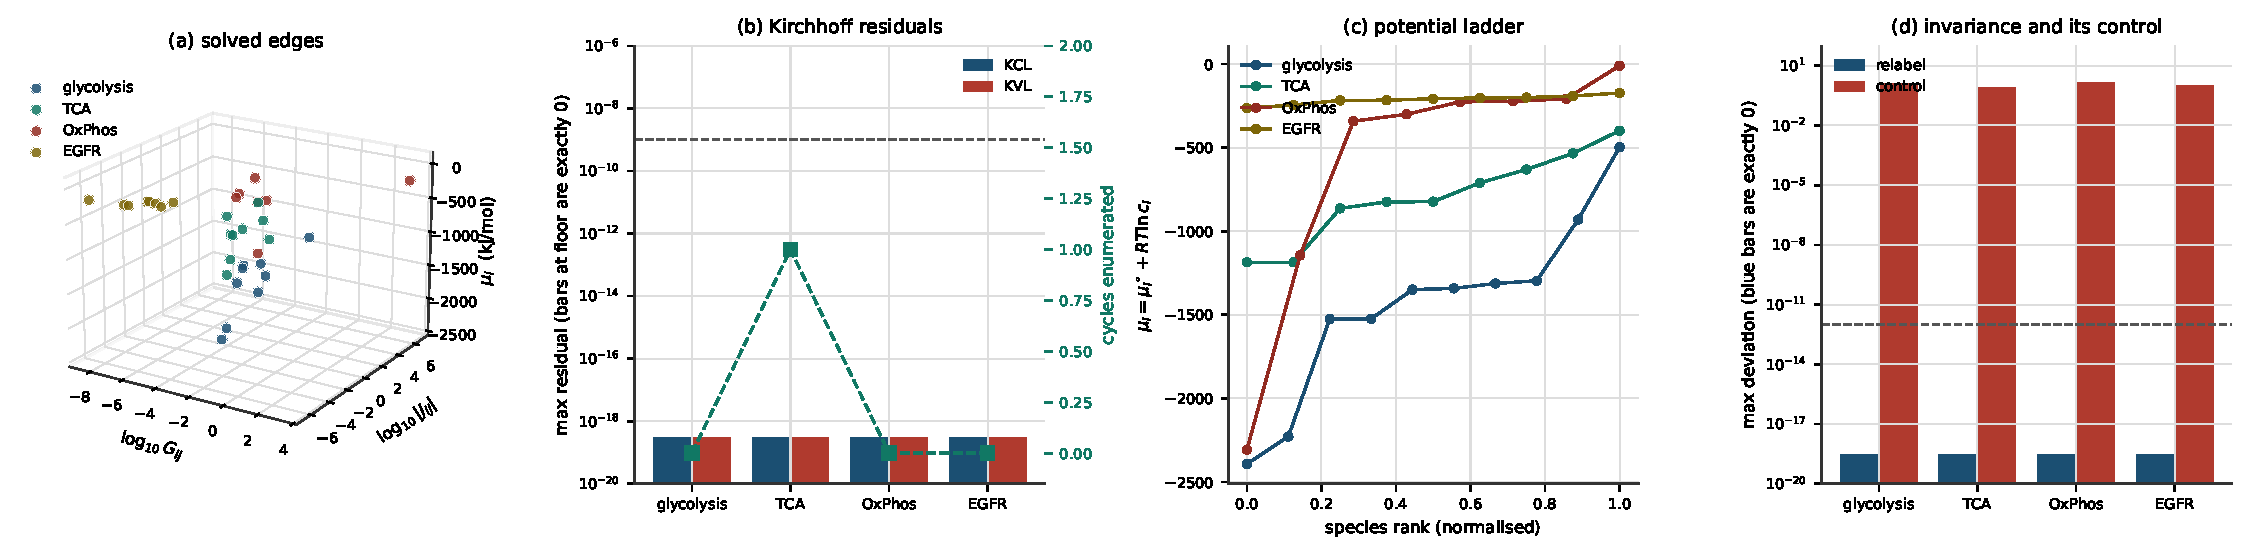
\includegraphics[width=\textwidth]{figures/panel_1_circuit.pdf}
  \caption[The circuit layer]{\textbf{The circuit layer.}
  (a) Every solved edge of all four networks in
  $(\log_{10} G_{ij}, \log_{10}|J_{ij}|, \mu_i)$: conductances span fourteen
  decades, so the circuit is stiff rather than uniform.
  (b) Kirchhoff residuals per network on a logarithmic axis; all bars are drawn
  at the floor because every residual is exactly zero. The right-hand axis gives
  the number of simple directed cycles enumerated, and it is the honest
  limitation of this check: only the citric-acid cycle contributes one, so the
  Wegscheider half of \cref{thm:kirchhoff} rests on a single cycle.
  (c) The potential ladder $\mu_i = \mu_i^\circ + RT\ln c_i$ against normalised
  species rank.
  (d) The invariance of \cref{prop:contact-determined} against its control:
  relabelling moves the contact map by nothing at all, permuting the underlying
  concentrations moves it by roughly $10^{0}$.}
  \label{fig:panel1}
\end{figure}

The consistency results hold as stated. Wegscheider residuals sit at machine
epsilon on every enumerated cycle, which is the check that cannot be fudged:
were it to fail, $\mu$ would not be a function on vertices and the circuit
representation would be inadmissible. Relabelling leaves the contact map fixed
exactly, while the control that permutes concentrations rather than labels moves
it by $0.80$ to $1.41$, so the invariance of
\cref{prop:contact-determined} is being tested rather than assumed. Step count
equals address length with zero variance at every depth from $2$ to $10$;
the equivalence of \cref{prop:sigma-partition} holds with no mismatches;
deleting the cache changes no output byte.

\begin{figure}[htbp]
  \centering
  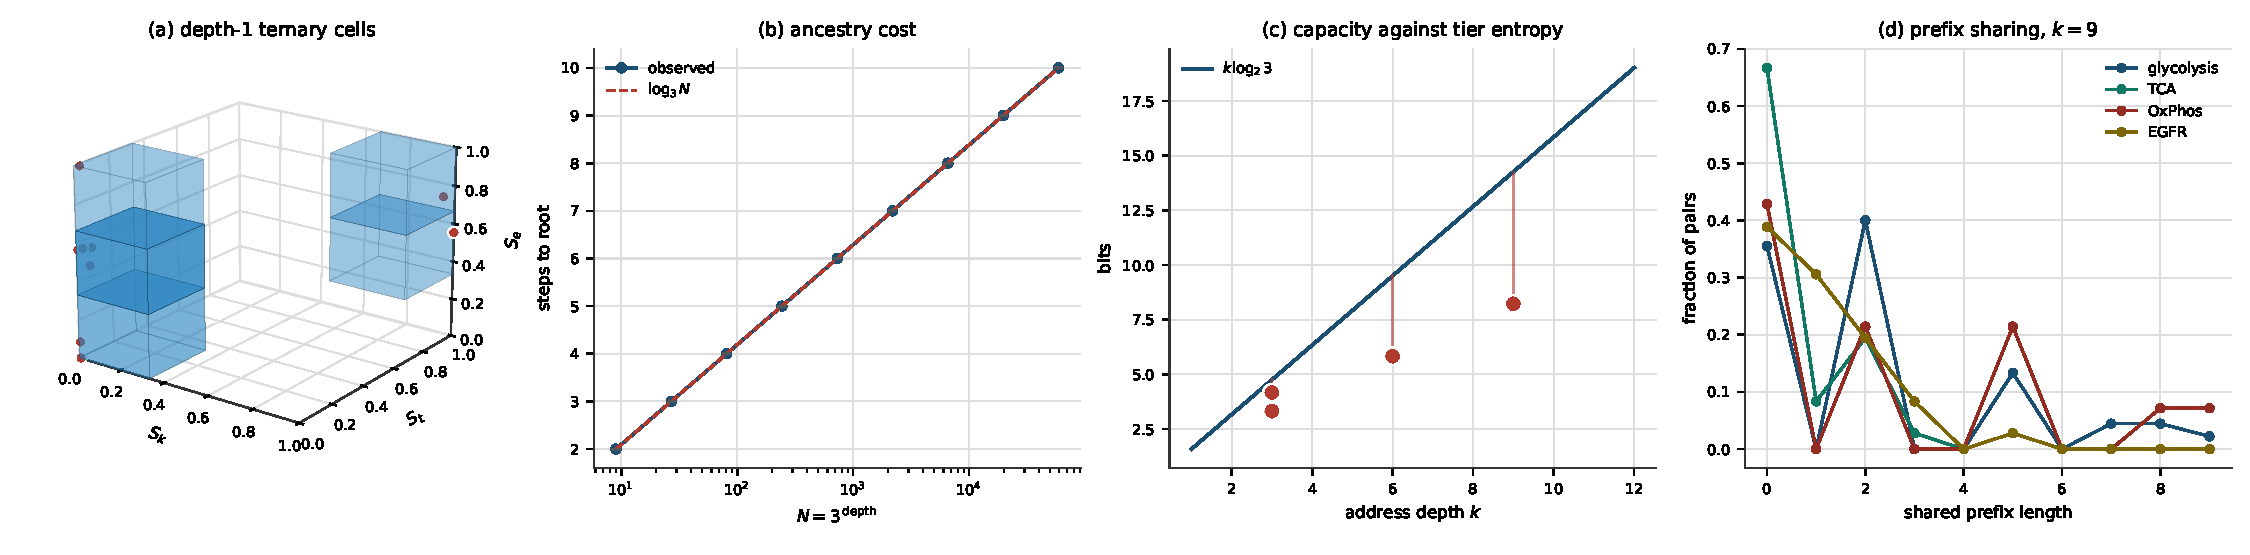
\includegraphics[width=\textwidth]{figures/panel_3_addressing.pdf}
  \caption[Addressing]{\textbf{Addressing.}
  (a) The depth-one ternary cells actually occupied by the four networks, drawn
  in the unit cube with opacity proportional to occupancy: the addressing scheme
  partitions $[0,1]^3$, but the coordinates populate a small part of it.
  (b) Ancestry cost. Observed steps to root against $N = 3^{\text{depth}}$ on a
  logarithmic axis, lying on $\log_3 N$ with zero variance at every depth --- the
  content of \cref{prop:notree}(ii), computed without materialising the trie.
  (c) Capacity $k\log_2 3$ against address depth, with the four tiers of the
  worked family plotted at their entropies; every tier sits below the line, which
  is the inequality of \cref{prop:capacity} holding with slack.
  (d) Distribution of shared prefix length over all species pairs at $k = 9$.
  Mass concentrated at short prefixes is what makes the address discriminating.}
  \label{fig:panel3}
\end{figure}

\begin{figure}[htbp]
  \centering
  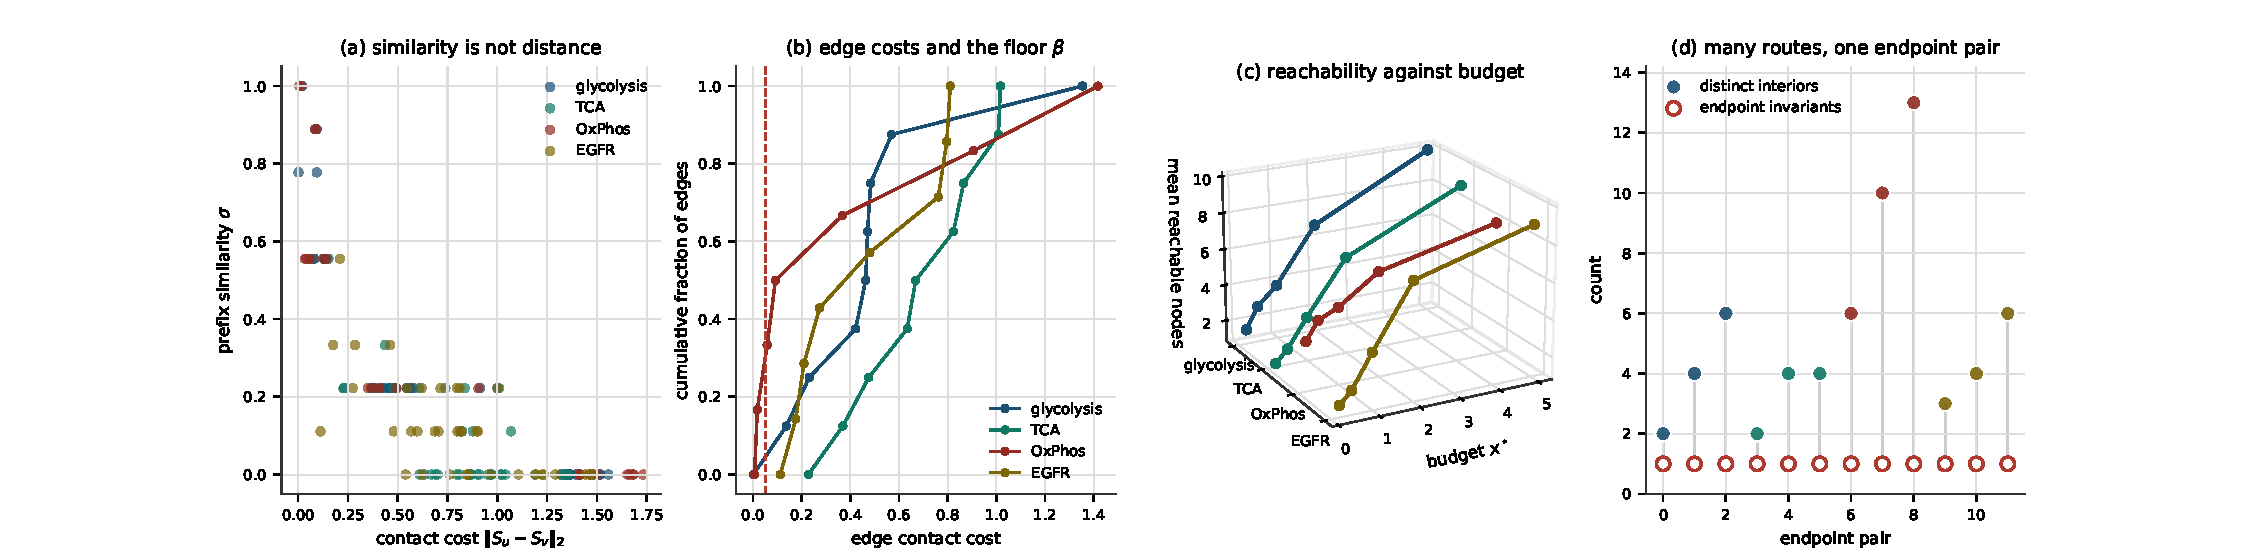
\includegraphics[width=\textwidth]{figures/panel_4_propagation.pdf}
  \caption[Propagation]{\textbf{Propagation.}
  (a) Prefix similarity $\sigma$ against contact cost $\lVert S_u - S_v\rVert_2$
  for every species pair. The relation is not monotone --- pairs at
  $\sigma = 0$ occur at every cost, and pairs at equal cost take most available
  $\sigma$ --- which is \cref{rem:sigma-not-metric} shown directly: $\sigma$
  reports a partition, not a distance.
  (b) Cumulative distribution of edge contact costs, with the floor $\beta$
  marked; the mass of edges above $\beta$ is what makes budgets bind.
  (c) Mean reachable nodes against budget $x^\star$ per network. Reachability
  grows with budget at a network-specific rate, so the budget is a real
  constraint rather than a formality.
  (d) For each endpoint pair, the number of distinct route interiors against the
  number of distinct endpoint invariants. Interiors proliferate; the invariant
  stays at one. This is \cref{thm:opacity}: the construction returns an
  equivalence class of routes, and increasing $k$ does not narrow it.}
  \label{fig:panel4}
\end{figure}

Two results are negative, and they are the informative ones.

\paragraph{The coordinate degenerates under a dominating species.}
On oxidative phosphorylation, $\Sk$ and $\St$ are exactly collinear:
each regresses on the other two axes at $R^2 = 1.000$. The cause is visible in
the inputs. Water at $\SI{55}{\mole\per\litre}$ exceeds the next-largest concentration
by roughly six orders of magnitude, so both max-normalisers in \cref{eq:coords}
collapse onto a two-valued indicator separating the water/ATP pair from
everything else, and the address carries about one axis of information instead
of three. Glycolysis sits close to the same edge at $R^2 = 0.989$. This is a
defect of the normalisation, not of the networks: \cref{eq:coords} divides by
network extrema and is therefore not robust to a species that dominates the
extremum. On the remaining three networks no axis is recoverable from the other
two, so the third axis is not redundant by construction --- which is the claim
(V3) actually makes --- but a practitioner should compute the axis regressions
before trusting a three-axis address on any given network.

\begin{figure}[htbp]
  \centering
  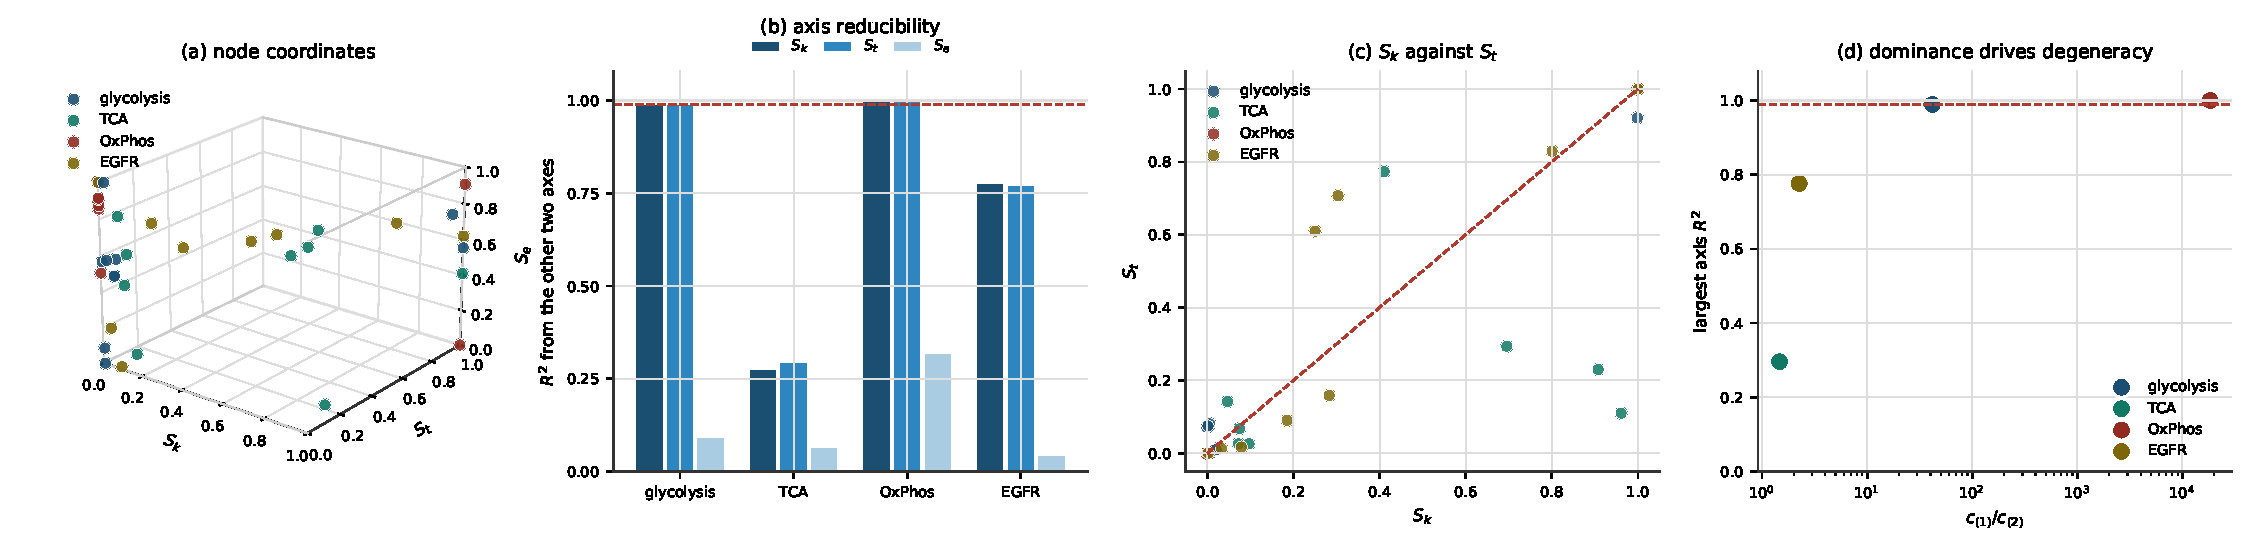
\includegraphics[width=\textwidth]{figures/panel_2_coordinate.pdf}
  \caption[The coordinate and its degeneracy]{\textbf{The coordinate, and where
  it degenerates.}
  (a) Every species of all four networks at its coordinate
  $(\Sk, \St, \Se)$ in the unit cube of \cref{eq:coords}.
  (b) Axis reducibility: $R^2$ from regressing each axis on the other two, with
  the $0.99$ line marked. Oxidative phosphorylation saturates on $\Sk$ and $\St$
  and glycolysis nearly does; the citric-acid cycle and the EGFR cascade do not.
  (c) The oxidative-phosphorylation collinearity shown without a regression:
  $\St$ against $\Sk$ collapses onto a two-valued indicator rather than
  spreading over the square.
  (d) The mechanism. Largest axis $R^2$ against the concentration dominance
  ratio $c_{(1)}/c_{(2)}$ on a logarithmic axis. Degeneracy tracks dominance:
  the two networks carrying a species that exceeds the next by orders of
  magnitude are the two whose coordinate collapses. Since \cref{eq:coords}
  divides by network extrema, this is a defect of the normalisation and not of
  the networks.}
  \label{fig:panel2}
\end{figure}

\begin{figure}[htbp]
  \centering
  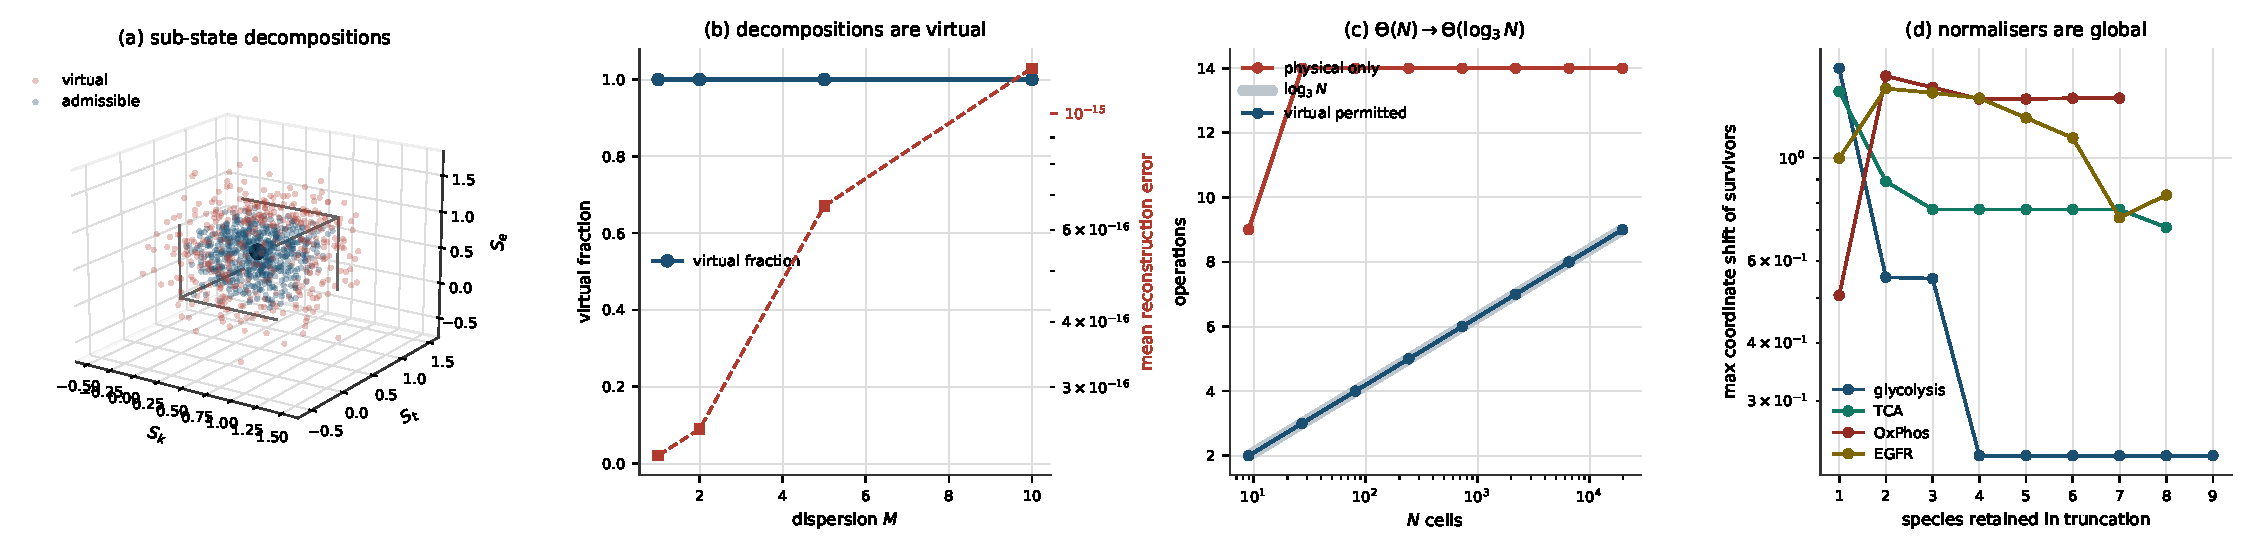
\includegraphics[width=\textwidth]{figures/panel_5_virtual.pdf}
  \caption[Virtual sub-states]{\textbf{Virtual sub-states and the collapse.}
  (a) One state (black) and its sub-state decompositions. Sub-states falling
  outside the unit cube (red) are virtual in the sense of
  \cref{thm:collapse} --- they are not themselves admissible coordinates, yet
  they average exactly to one that is.
  (b) Virtual fraction against dispersion $M$, with mean reconstruction error on
  the right-hand axis. Every decomposition at every dispersion is virtual, and
  reconstruction holds to $10^{-15}$: the averaging identity is exact while the
  parts are unphysical.
  (c) The collapse of \cref{cor:speedup}. Operations against $N$ cells,
  logarithmic in $N$; permitting virtual sub-states tracks $\log_3 N$ (drawn as
  the wide underlay, which the data lies on) where the physical-only count
  saturates.
  (d) Why the normalisers are global. Truncating a network to its largest
  species shifts the coordinates of the survivors, by up to order unity for
  small truncations --- so a coordinate is a statement about a network, not
  about a species in isolation.}
  \label{fig:panel5}
\end{figure}

\paragraph{The panel floor is two, not three.}
\Cref{thm:discrimination} holds exactly: across all subsets of the available
observables, separating every pair and separating the whole state set coincide
with no exceptions in either direction. The floor asserted by the earlier
reading of \cref{cor:three} does not survive. Exhaustive search returns
$\chi = 2$, attained uniquely by absorption together with oxidation state, for
the reason given in \cref{rem:floor-computed}. We report this rather than
adjusting the state table to recover the number three, since a state table
tuned until the answer comes out right is the failure mode
\cref{rem:control-refused} describes. What survives is the substantive claim,
and it is the one worth carrying: disjointness of observables buys resolution,
cardinality does not, and the floor must be computed per system.

\begin{figure}[htbp]
  \centering
  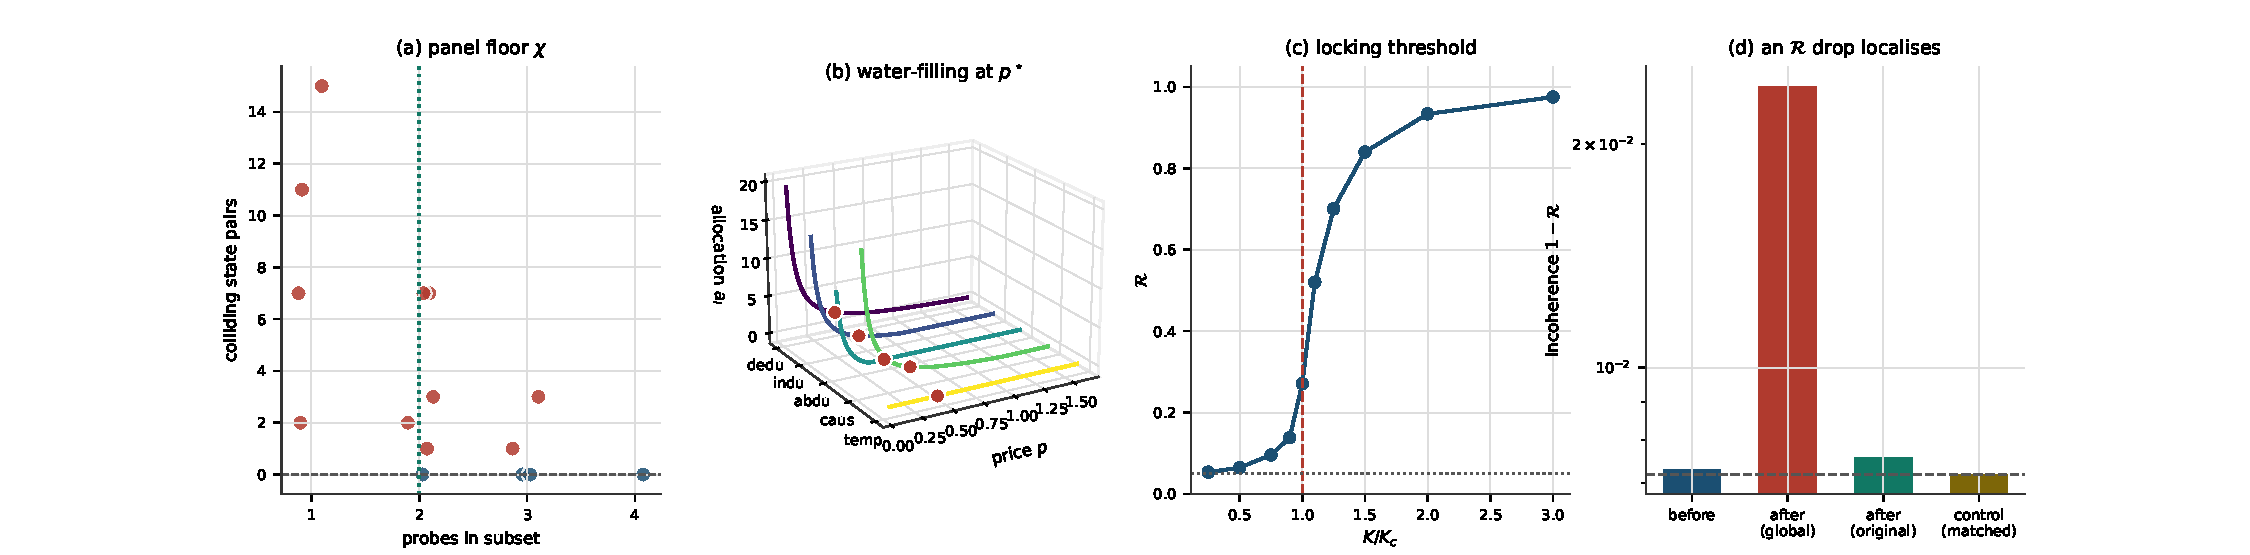
\includegraphics[width=\textwidth]{figures/panel_6_panel_layer.pdf}
  \caption[The panel layer]{\textbf{The panel layer.}
  (a) Colliding state pairs for every subset of the four observables, against
  subset size. Subsets reaching zero collisions (blue) are exactly those that
  separate the whole state set, with no exceptions in either direction, which is
  \cref{thm:discrimination}. The floor $\chi = 2$ is marked; size alone does not
  determine separation, since some three-element subsets still collide.
  (b) Water-filling. Allocation against price for each reasoner, with the
  solution at the single shadow price $p^\star$ marked. Allocations are graded
  and the low-weight, high-cost reasoner sits at the dropout boundary of
  \cref{cor:graded} rather than being excluded by a separate rule.
  (c) The locking threshold of \cref{thm:lock}. Order parameter against
  $K/K_c$ with $K_c$ computed rather than fitted, and the finite-$M$ incoherent
  floor $1/\sqrt{M}$ marked; the transition occurs at the predicted place.
  (d) Localisation, plotted as incoherence $1-\mathcal{R}$ on a logarithmic axis
  because the whole effect lies in the third decimal. Admitting a mismatched
  newcomer drops the global order parameter, the order parameter restricted to
  the original members is essentially unmoved, and the matched-newcomer control
  does not drop at all. The dashed line is the bound of
  \cref{prop:localisation}.}
  \label{fig:panel6}
\end{figure}

One further correction belongs in the record. The discrimination experiment
initially modelled each probe as a bin label --- band position rounded to the
instrument's resolving power --- and reported that absorption alone separates
all seven states. That was an artefact: rounding separates two readings
whenever they straddle a bin edge, however close they are, so
$\SI{417}{\nano\metre}$ and $\SI{418}{\nano\metre}$ came apart while
genuinely-resolved pairs did not. A resolving power is a proximity relation,
not a partition. Rewriting each probe as the separation relation it actually
denotes produced exactly the two documented collisions.

\section{Limitations}
\label{sec:limits}

\paragraph{Steady state is assumed throughout.}
\Cref{thm:kirchhoff} and everything after it hold at steady state.
The recovered graph is time-invariant, and no claim is made about transient
dynamics, oscillatory regimes, or systems far from stationarity. A network whose
biology is in its transients is outside scope.

\paragraph{Ideal-solution chemical potentials.}
\Cref{eq:mu} omits activity coefficients. For crowded intracellular conditions
this is a real approximation, and the coordinate of \cref{eq:coords} inherits
its error. The error enters $\Se$ directly and $\Sk,\St$ through the flux and
conductance sums.

\paragraph{Mechanism is not recoverable.}
By \cref{thm:opacity} the construction returns an equivalence class of routes.
Where the route is the scientific object --- mechanistic enzymology, isotope
tracing --- this is the wrong instrument, and increasing $k$ does not help.

\paragraph{Coordinates are network-relative.}
The normalisers in \cref{eq:coords} are network extrema, so addresses are not
comparable across networks without a shared normalisation. Comparing addresses
computed under different networks is the most likely misuse.

\paragraph{The normalisation is not robust to a dominating species.}
Dividing by a network extremum makes the coordinate fragile when one species
carries that extremum by orders of magnitude. \Cref{sec:results} exhibits the
failure: on oxidative phosphorylation, water at bulk concentration collapses
$\Sk$ and $\St$ into the same two-valued indicator, giving exact collinearity
and reducing an address that nominally carries three axes to about one. A rank
or logarithmic normalisation would likely be better behaved, but we have not
established that and do not use it, so the practical guidance is to compute the
axis regressions of (V3) per network and to distrust the address where an axis
is recoverable from the others.

\paragraph{Kinetic parameters bound accuracy.}
\Cref{prop:contact-determined} says the graph is a function of the kinetic
description. Where $k_{ij}$ or $c_i$ are wrong, the graph is wrong in a way no
internal check detects, because internal consistency is preserved under
consistent error.

\paragraph{Two constants are unreconciled.}
Whether the contact floor $\beta$ of \cref{ass:floor} and the numerical
resolution floor of the coordinate construction are the same constant under
rescaling is open. We have not established it and do not use it.

\paragraph{Metric compatibility is unverified.}
The Euclidean contact cost of \cref{eq:contact} and the information-geometric
metric natural on a space of normalised triples \citep{Amari2016} need not agree.
We use Euclidean distance because the reference implementation does, and flag
that no compatibility result is claimed.

\paragraph{The panel results are structural, not empirical.}
\Cref{thm:waterfill,thm:lock,prop:localisation} are theorems about the panel
model. That a panel of reasoners built this way outperforms a single reasoner on
a biological question is not established here and would require the validation
of \cref{sec:validation} run end to end on a real network.

\section{Conclusion}

The construction reduces to three identifications and one accounting.

The identifications: a steady-state reaction network \emph{is} a resistive
circuit (\cref{thm:kirchhoff}); the solved circuit's per-species coordinate
\emph{is} a base-3 address under interleaved digitisation
(\cref{def:encoding}), so that ancestry and similarity are both prefix
arithmetic (\cref{prop:notree}, \cref{prop:sigma-partition}); and the causal
knowledge graph \emph{is} the circuit's propagation operator evaluated at the
resting process (\cref{thm:catalogue}). Nothing is asserted into the graph;
it is recovered, and recomputing returns it.

The accounting: backward interrogation costs $\Theta(\log_3 N)$ and forward
construction costs $\Theta(N)$, with the gap attributable entirely to virtual
sub-states, which are legitimate in the first case and provably unavailable in
the second (\cref{thm:collapse}, \cref{cor:speedup},
\cref{thm:forward-asymmetry}). Resident state is $O(1)$ in addressable objects,
bought by recomputation rather than compression, and worth having only where the
query set is not known in advance (\cref{prop:resident},
\cref{rem:honest}).

Two consequences are worth separating from the machinery because they change how
results are read. First, an edge of the recovered graph names a class of
mechanisms and not a mechanism (\cref{thm:opacity}); this is a limitation, and
stating it as a theorem is the only honest way to carry it. Second, two
derivations that share endpoints and fixed point cannot contradict each other,
so their divergence measures resolved extent rather than truth
(\cref{thm:amalgamation}, \cref{cor:reclassify}) --- conditional on a
convergence check that must actually be performed.

What the construction does not supply is accuracy. \Cref{prop:contact-determined}
guarantees the graph is a faithful function of the kinetic description it was
given, and says nothing whatever about whether that description is right.

The validation of \cref{sec:results} bears this out in both directions. The
consistency claims hold to machine precision, and two claims that were stated
too strongly do not: the coordinate degenerates on a network containing a
species at bulk concentration, and the panel floor is a computed property of the
state and observable sets rather than the constant three. Both were found by
tests built to be capable of failing, which is the only reason they were found
at all.

\bibliographystyle{plainnat}
\bibliography{references}

\end{document}
